% !TeX root = ../main.tex
\chapter{原学习配额变体的模型与训练}
\label{app:legacy-learning}
% Local list pagination: keep the final appendix-table entry on the same list page.
\addtocontents{lot}{\protect\enlargethispage{2\baselineskip}}
本附录保留原SF-HLM学习配额变体的推导。其CompleteQuotaPPO、最多16次匹配和教师初始化属于原协议；第五章主方法为解析缓存混合＋能耗定价，不使用该PPO作为在线执行器。此处的二值超时字典序证明也不用于连续混合分数的最优性论证。共同移动前模型见第\ref{cha:ch5-sfhlm}章。

\section{配额分解与条件化字典序匹配}
\label{legacy:sec:ch5-matching}

\subsection{配额空间与分配空间的关系}

若每个请求最多有六个合法执行目标，直接分配空间至多包含 $6^R$ 个组合。SF-HLM 首先考虑整数配额空间
\begin{equation}
 \mathcal{N}_R=\left\{\mathbf{n}\in\mathbb{Z}_{\ge0}^{6}:\sum_{j=0}^{5}N_j=R\right\},
 \qquad |\mathcal{N}_R|=\binom{R+5}{5}.
 \label{legacy:eq:ch5-quota-space}
\end{equation}
这个数量是忽略质量掩码后的配额数上界；掩码会排除某些无法由合法请求组成的配额。配额表示保留了算力共享所需的关键统计量，使负载相关项在给定 $\mathbf N$ 后成为已知常数。与此同时，它没有强迫同样大小的任务交换身份，也没有按配额均匀随机分配请求，具体任务依然交由条件匹配选择。

配额分解的作用并非声称整个问题已变为低复杂度精确问题。式~\eqref{legacy:eq:ch5-quota-space} 仍随批量规模增长，在线预算不允许穷举。其实际优势是把复杂的两种决策分开：图策略在配额层选择值得尝试的负载组织，确定性匹配器在该组织内利用请求差异寻找分配。学习器不必逐个生成全部请求的完整组合，也不必从回报中独立重新学习指派求解器已经能够表达的条件最优结构。

\subsection{容量槽展开与合法指派}

给定配额 $\mathbf N$，将每个节点 $j$ 展开为 $N_j$ 个容量槽。全部槽的集合为 $\mathcal S(\mathbf N)$，大小恰好为 $R$；槽 $s$ 对应的执行节点记为 $j(s)$。令 $y_{ms}\in\{0,1\}$ 表示请求 $m$ 是否占据槽 $s$，则条件匹配满足
\begin{equation}
 \sum_{s\in\mathcal S}y_{ms}=1,\qquad
 \sum_{m\in\mathcal R}y_{ms}=1,\qquad
 y_{ms}=0\quad\bigl(j(s)\notin\mathcal J_m\bigr).
 \label{legacy:eq:ch5-slot-constraints}
\end{equation}
同一节点的容量槽具有相同边成本，但分别只能接收一个请求。由一一指派得到的分配自动满足式~\eqref{eq:ch5-assignment-feasibility}，且每个节点最终恰好接收 $N_j$ 个请求。图~\ref{legacy:fig:ch5-slots} 展示配额、容量槽与请求身份的关系。

\begin{figure}[!htbp]
 \centering
 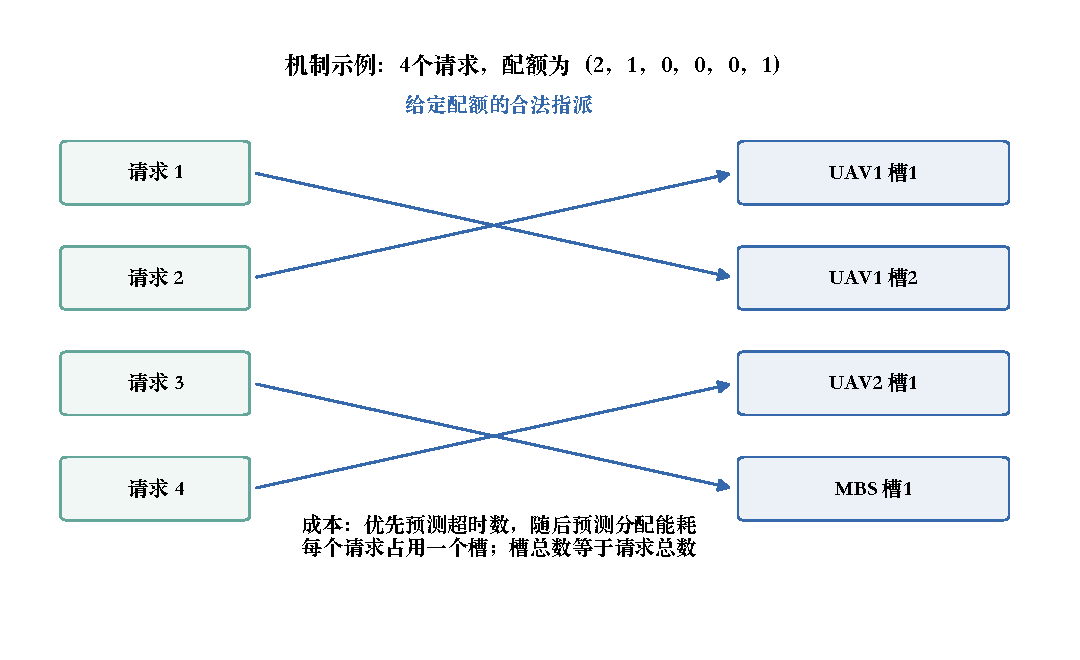
\includegraphics[width=0.95\textwidth]{../docs/figures/图5-2_配额与容量槽匹配}
 \bicaption{固定配额的容量槽展开与请求匹配。示意图用于解释算法结构，不是实测任务分配}{Capacity-slot expansion and request assignment under fixed quotas; a conceptual illustration}
 \label{legacy:fig:ch5-slots}
\end{figure}

配额可行性由完整指派确认。各节点的合法边数只是必要条件：若多节点依赖同一小部分请求，仍可能无法同时填满容量槽。非法边设无穷成本，使用 SciPy 线性指派接口\cite{virtanen2020scipy}求解，其修改的 Jonker--Volgenant 方法背景见文献\cite{crouse2016assignment}。返回后检查边合法性与节点数量守恒；不可行调用同样计入预算，并保留已有最好方案。

\subsection{字典序目标的标量化与严格等价性}

给定 $\mathbf N$，先计算全部合法边的预测能耗，令
\begin{equation}
 E_{\max}(\mathbf N)=\max_{m,j:\,j\in\mathcal J_m}\widehat E_{mj}(N_j),
 \qquad \widetilde E_{mj}=\frac{\widehat E_{mj}(N_j)}{\max(E_{\max},\epsilon_E)}.
 \label{legacy:eq:ch5-energy-normalization}
\end{equation}
实现用极小正数 $\epsilon_E$ 防止所有能耗为零时除零。合法边能耗非负且 $\widetilde E_{mj}\le1$，因此任何完整合法指派的归一化能耗和均处于 $[0,R]$。构造容量槽成本
\begin{equation}
 C_{ms}=(R+1)\mathbf1\{\widehat T_{m,j(s)}(N_{j(s)})>D_m\}
       +\widetilde E_{m,j(s)},
 \label{legacy:eq:ch5-slot-cost}
\end{equation}
非法边成本为无穷。线性指派求解
\begin{equation}
 \min_{\mathbf y}\sum_{m,s}C_{ms}y_{ms}
 \quad\text{满足式~\eqref{legacy:eq:ch5-slot-constraints}}.
 \label{legacy:eq:ch5-linear-assignment}
\end{equation}
权重 $R+1$ 随当前批量规模确定，不使用任意调试的超时惩罚常数。

下面说明式~\eqref{legacy:eq:ch5-linear-assignment} 与固定配额下的 $(M,E)$ 字典序最小化等价。任取两个完整合法指派 $\mathbf y^{a},\mathbf y^{b}$，若 $M_a\ge M_b+1$，其标量目标差满足
\begin{equation}
 \mathcal C_a-\mathcal C_b
 =(R+1)(M_a-M_b)+\widetilde E_a-\widetilde E_b
 \ge(R+1)-R=1>0.
 \label{legacy:eq:ch5-lex-proof}
\end{equation}
因此，无论能耗怎样变化，多一个预测超时的分配都不可能取得更小的标量成本。若 $M_a=M_b$，标量目标只比较归一化能耗；固定配额内归一化比例相同，故该比较与原始能耗大小完全一致。这证明求解器首先最小化预测超时数，再在最少超时的分配中最小化预测分配能耗。

上述条件最优性适用于\emph{给定配额、固定预测信息及合法指派域}。能耗上限在求解后筛选：若最少预测超时的匹配超出上限，该候选被拒绝，不再搜索该配额下其他受限指派。因而，条件匹配提供可利用的精确子结构，配额搜索及能耗约束下的整体性能仍需独立评价。

\subsection{预测能耗参照与保底方案}

先按固定请求顺序构造原始贪心分配 $\mathbf x^{\mathrm g}$。处理一个请求时，贪心按已分配目标数估计加入后的自身时延，依次以自身时延、自身分配能耗和动作编号决胜。共同能耗参照由该\emph{原始贪心的最终批量重评估}确定：
\begin{equation}
 E_{\mathrm{cap}}=1.05E(\mathbf x^{\mathrm g}).
 \label{legacy:eq:ch5-energy-cap}
\end{equation}
普通修复、配额学习、启发式和强随机均使用同一状态下的这个上限。它不是各方法自己的初始分配乘 $1.05$，从而避免某个方法由于初始方案能耗偏高而获得更宽松的筛选空间。

普通修复以一次请求迁移为邻域，在最多 $128$ 次候选评价内寻找字典序改进。若已有学习下层提出的初始分配超出共同上限，先回到原始贪心，再开展修复；若未超限则从其提案出发。配额方法从共同贪心加修复的保底进入，并对该保底配额作一次条件匹配。候选只有在合法且预测分配能耗不超过 $E_{\mathrm{cap}}$ 时才能成为当前搜索状态；最好方案由所有已接受方案中的 $(M,E)$ 决定。

由此，最终分配保持完整、质量合法且预测能耗不超过共同上限，最好预测目标不劣于共同保底。该性质涉及分配预测量；环境中的真实缓存和请求执行仍影响实际结果，飞行、悬停及无线能量传输也未包含在 $E(\mathbf x)$ 内。因此，实验另行统计完整 UAV 机队能耗。

\section{有限预算配额搜索与二部图策略}
\label{legacy:sec:ch5-search}

\subsection{当前状态、最好状态与动作空间}

搜索的内部步号记为 $\ell$，区别于环境时隙 $t$。一个环境时隙内可以进行若干次配额迁移，但只有最终保留的分配进入环境。当前配额、当前分配与其预测目标分别记为 $\mathbf N^{(\ell)},\mathbf x^{(\ell)},F^{(\ell)}$；最好分配与目标记为 $\mathbf x^{*(\ell)},F^{*(\ell)}$。允许搜索经过比最好方案更差的当前方案，使策略能够跨越只接受即时改进的局部限制；实际执行则不受这些较差中间方案直接影响。

完整搜索过程的状态可写为
\begin{equation}
 S_\ell=(\mathcal R,\mathbf N^{(\ell)},\mathbf x^{(\ell)},\mathbf x^{*(\ell)},\mathcal V_\ell,B_\ell),
 \label{legacy:eq:ch5-full-search-state}
\end{equation}
$\mathcal V_\ell$ 为已尝试配额集合，$B_\ell$ 为剩余调用预算，请求预测量在单次搜索内固定。条件匹配与访问更新定义搜索转移。策略读取当前与最好分配的图编码及有效动作掩码，这些输入构成完整搜索状态的可计算观测。有限搜索的性能通过对应对照评价。

配额动作集合为
\begin{equation}
 \mathcal A=\{\mathrm{STOP}\}\cup
 \{(i,j,k):i,j\in\mathcal J,\ i\ne j,\ k\in\{1,2,4\}\},
 \qquad |\mathcal A|=91.
 \label{legacy:eq:ch5-action-space}
\end{equation}
转移动作仅改变节点任务数量：
\begin{equation}
 \mathbf N'=\mathbf N^{(\ell)}-k\mathbf e_i+k\mathbf e_j.
 \label{legacy:eq:ch5-quota-transfer}
\end{equation}
这里的“转移 $k$ 个任务”是配额变动，不是预先指定 $k$ 个请求的身份。新配额的具体分配重新由条件匹配给出，可能改变多个请求的目标。因此，一次配额动作能够触发批量重组，而不是仅对一个被选中的任务作局部替换。

有效动作掩码同时要求 $N_i\ge k$、新配额没有访问过、各节点配额不大于其合法边数。最后一项只是必要条件，完整可行性由匹配求解检查。STOP 始终有效，使没有可行迁移时策略也能合法终止。失败的匹配配额同样加入访问集合，避免重复耗费预算。采样时掩码属于保存的搜索状态，重算概率时不得根据更新后的访问集合重新生成它。

初始条件匹配占用一次调用，整个搜索最多 $16$ 次匹配，因此普通非空批次最多再尝试 $15$ 次配额迁移。策略可以提前 STOP，也可能因为调用预算耗尽而终止；空批次不消耗匹配预算。搜索预算是求解器调用数，而不是动作数、成功迁移数或模型前向次数。该定义使不可行候选与超能耗候选也承担实际计算费用，便于与启发式和强随机保持共同预算。

\subsection{请求、边与节点特征}

图~\ref{legacy:fig:ch5-graph} 表示每个搜索状态的二部图。请求是左侧节点，六个执行节点是右侧节点，质量合法动作构成边。请求输入保留截止时间、计算量、输入大小和源节点；边输入描述请求放在该目标后的预测路径和负载；节点输入同时描述当前与最好方案的服务压力。区分当前与最好状态很重要：如果只编码最好方案，策略无法知道自己正在从哪个较差入口继续迁移；如果只编码当前方案，又无法知道已经保留的执行质量和剩余改进空间。

\begin{figure}[!htbp]
 \centering
 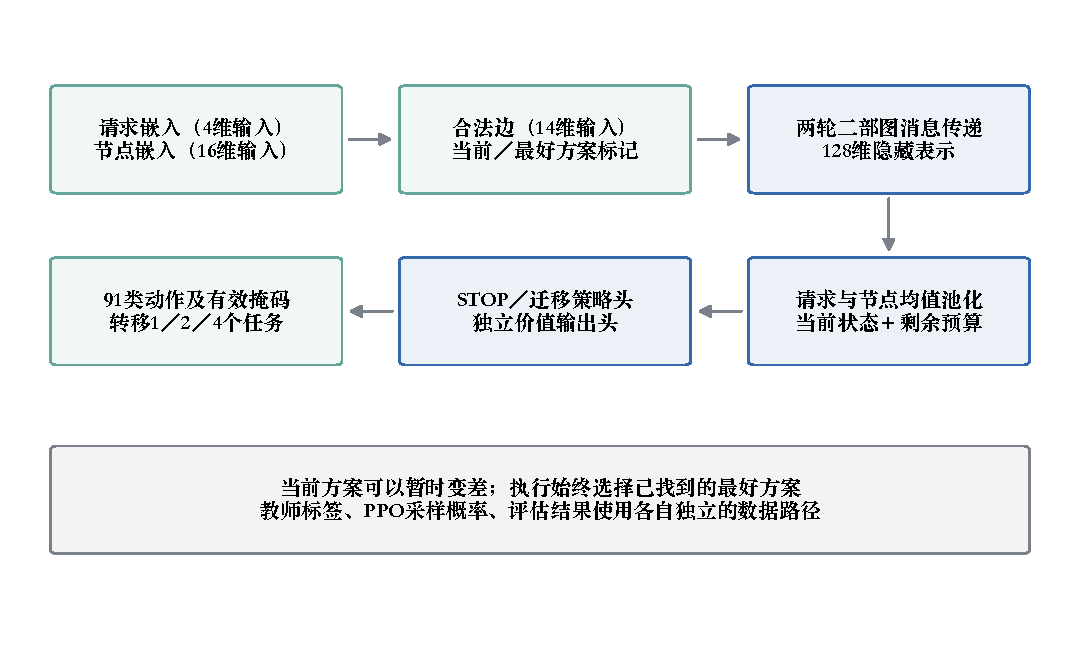
\includegraphics[width=0.98\textwidth]{../docs/figures/图5-3_二部图网络与搜索状态}
 \bicaption{请求--执行节点二部图、当前与最好状态编码及配额动作头。非法边和填充请求在消息聚合中屏蔽}{Request--execution-node graph, current/best state encoding and quota action heads}
 \label{legacy:fig:ch5-graph}
\end{figure}

请求特征 $\mathbf v_m\in\mathbb R^4$ 为
\begin{equation}
 \mathbf v_m=\left[\min(D_m,10),\ \frac{\log(1+C_m)}{30},\
 \frac{\log(1+L_m)}{20},\ \frac{u_m}{5}\right].
 \label{legacy:eq:ch5-request-features}
\end{equation}
秒、CPU 周期和字节数各自在进入网络前作固定尺度变换。变换用来控制数值范围，不改变指派预测器使用的原始量。尤其是网络中截止时间截断到 $10$ 的表示，不意味着真实截止时间判断也被截断。

合法边 $\mathbf z_{mj}\in\mathbb R^{14}$ 的前十二项依次为：$b_{mj}/D_m$、$w_{mj}/D_m$、$\log(1+e_{mj})/20$、$\log(1+c_{mj})/30$、当前 $N_j/R$、截断后的 $\widehat T_{mj}/D_m$、归一化截止期余量、允许负载阈值的归一化值、MBS 标记、缓存信念、目标容量的对数表示和源节点标记。最后两项为当前分配与最好分配是否经过该边的二元标记。非法边的特征置零，并在后续聚合中屏蔽。负载阈值来自 $(D_m-b_{mj})/\max(w_{mj},10^{-12})$，只作为网络观测特征；最终方法没有把临界阈值扩展为新的动作集合。

令请求在指定分配中的归一化余量为 $m_m=1-\widehat T_m/D_m$。每个节点的六项服务摘要为：接收数量占批次比例、节点内预测超时比例、平均余量、最小余量、释放一个请求可能救回的请求数占批次比例、节点分配能耗占参照比例。释放救回的判定为
\begin{equation}
 b_{mj}+w_{mj}\max(N_j-1,1)\le D_m
 < b_{mj}+w_{mj}N_j,
 \label{legacy:eq:ch5-release-rescue}
\end{equation}
且只对 UAV 目标计算。摘要既描述节点已经承担的请求，也提示减少该节点负载可能影响的其他请求；它没有读取真实执行成功标签。

当前与最好方案分别生成六项摘要，拼接当前配额比例、剩余匹配预算比例、当前和最好预测超时占批次比例，得到 $\mathbf u_j\in\mathbb R^{16}$。所有比例在空批次处理时采用正分母保护；空节点摘要为零。平均和最小余量截断到 $[-10,1]$，边时延比上限为 $10$，容许负载特征截断到 $[-1,2]$。这些固定处理约束输入数值而不改变真实请求数量、目标可行性或实际性能评价。

\subsection{两层消息传递与置换结构}

分别用 MLP 将请求、节点与边特征映射为 $h=128$ 维嵌入，记为 $\mathbf h_m^{(0)},\mathbf g_j^{(0)},\mathbf e_{mj}$。每个 MLP 由线性层、LayerNorm、ReLU 和输出线性层组成。两轮消息传递中，第 $q$ 层合法边消息为
\begin{equation}
 \mathbf m_{mj}^{(q)}=\psi_q\bigl([
 \mathbf h_m^{(q)},\mathbf g_j^{(q)},\mathbf e_{mj}]\bigr),
 \qquad j\in\mathcal J_m.
 \label{legacy:eq:ch5-message}
\end{equation}
$\psi_q$ 在所有合法边共享参数，非法边消息恒为零。请求侧和节点侧各按合法邻居取均值，并分别更新：
\begin{equation}
 \begin{aligned}
 \overline{\mathbf m}_m^{(q)}&=
 \frac{\sum_{j\in\mathcal J_m}\mathbf m_{mj}^{(q)}}{\max(|\mathcal J_m|,1)},
 &\mathbf h_m^{(q+1)}&=\rho_q([\mathbf h_m^{(q)},\overline{\mathbf m}_m^{(q)}]),\\
 \overline{\mathbf m}_j^{(q)}&=
 \frac{\sum_{m:\,j\in\mathcal J_m}\mathbf m_{mj}^{(q)}}{\max(|\{m:j\in\mathcal J_m\}|,1)},
 &\mathbf g_j^{(q+1)}&=\nu_q([\mathbf g_j^{(q)},\overline{\mathbf m}_j^{(q)}]).
 \end{aligned}
 \label{legacy:eq:ch5-message-update}
\end{equation}
$q=0,1$，两层使用各自参数。批量训练时，请求图填充到同一批中的最大请求数；填充请求嵌入与消息均屏蔽，均值分母只计算真实合法邻居。

完成两层更新后，对真实请求取均值 $\overline{\mathbf h}$，对六个节点取均值 $\overline{\mathbf g}$。转移动作 $(i,j,k)$ 的分数由源节点、目的节点、请求池化表示和迁移量独热编码构成：
\begin{equation}
 z_{ijk}=f_{\mathrm{move}}([\mathbf g_i^{(2)},\mathbf g_j^{(2)},
                  \overline{\mathbf h},\operatorname{onehot}(k)]),\qquad
 z_{\mathrm{stop}}=f_{\mathrm{stop}}([\overline{\mathbf h},\overline{\mathbf g}]).
 \label{legacy:eq:ch5-action-heads}
\end{equation}
价值头同样使用 $[\overline{\mathbf h},\overline{\mathbf g}]$。掩码 logits 形成分类分布，训练时采样，评估时取最大分数动作。共享边函数与均值聚合对一致的请求排列保持不变，节点身份、源编号及合法域则仍作为显式输入。

这一网络用消息传递表达“同一个请求的替代目标”和“同一个节点上可竞争请求”的关系。它不采用多头注意力加权聚合，下层所有合法邻居的消息使用均值。SF-HLM 因而由上层注意力聚合与下层二部图 MLP 两种结构组成。可变请求数量由图表示和填充掩码处理，而六节点动作头保持固定，这使模型在冻结跨 UE 数量评价时无需增加动作维数。

\subsection{搜索奖励与最好方案不变量}

一次非停止迁移后，令最好预测超时与能耗从 $(M_{\ell-1}^{*},E_{\ell-1}^{*})$ 更新到 $(M_\ell^{*},E_\ell^{*})$，训练奖励定义为
\begin{equation}
 r_\ell=M_{\ell-1}^{*}-M_\ell^{*}
 +0.1\frac{E_{\ell-1}^{*}-E_\ell^{*}}{\max(E_{\mathrm{cap}},10^{-12})}-0.001.
 \label{legacy:eq:ch5-search-reward}
\end{equation}
奖励评价保留的最好方案，而非较差当前方案；一次没有改进的匹配尝试仍得到 $-0.001$ 的计算惩罚。STOP 奖励为零。预测超时减少具有主要作用，能耗项在共同上限下表达较小的平滑偏好，调用惩罚为节约搜索提供信号。这个搜索奖励服务于单时隙组合求解，与环境中的轨迹奖励和真实 DSR 是不同对象。

采用无折扣的有限搜索回报，若本次搜索进行了 $L$ 次非停止迁移，式~\eqref{legacy:eq:ch5-search-reward} 的差分项可望远镜求和：
\begin{equation}
 \sum_{\ell=1}^{L}r_\ell
 =M_0^*-M_L^*+0.1\frac{E_0^*-E_L^*}{\max(E_{\mathrm{cap}},10^{-12})}-0.001L.
 \label{legacy:eq:ch5-reward-telescope}
\end{equation}
$0$ 对应完成共同保底与初始匹配后的状态，初始匹配本身不产生一次迁移奖励。因此，训练在已有保底质量上权衡进一步改善与额外尝试，不奖励重复返回同一配额，也不把较差中间状态的真实执行结果回流到环境。

\begin{algorithm}[!htbp]
 \caption{SF-HLM 单时隙配额搜索与条件匹配}
 \label{legacy:alg:ch5-online}
 \KwIn{移动前请求行、质量合法域、冻结图策略 $\pi_\theta$；匹配预算 $16$，普通修复预算 $128$}
 \KwOut{全部已接纳请求的合法分配}
 构造原始贪心 $\mathbf x^{\mathrm g}$ 并计算 $E_{\mathrm{cap}}=1.05E(\mathbf x^{\mathrm g})$\;
 在共同上限内普通修复，初始化当前与最好分配\;
 根据保底配额执行初始条件匹配，计入一次匹配调用\;
 若候选合法、低于上限且目标更好，更新保留方案\;
 \While{批次非空、匹配调用未耗尽且搜索未停止}{
  编码当前/最好二部图及采样时掩码\;
  由图策略选择 STOP 或配额迁移 $(i,j,k)$\;
  \eIf{选择 STOP}{终止搜索\;}{
   生成守恒配额，记录已访问配额并计入一次匹配调用\;
   求解该配额的条件字典序匹配\;
   若匹配合法且满足共同能耗上限，更新当前方案\;
   若当前方案优于保留目标，更新最好方案\;
  }
 }
 将最好方案映射回各源 UAV 的请求动作，输出完整分配\;
\end{algorithm}

\subsection{计算量、终止条件与实现校验}

固定配额下的稠密成本矩阵为 $R\times R$，常规指派的时间量级为 $O(R^3)$、存储量级为 $O(R^2)$，实际实现与稀疏结构影响常数。图网络每轮处理至多 $6R$ 条边，在六节点与固定宽度下对请求数近似线性。完整在线时间还包括观测准备、普通修复、至多 $16$ 次匹配、动作映射及消息序列化。

调用预算保证有限搜索终止。有效迁移消耗匹配预算，访问去重避免重复，STOP 可提前结束，最终返回共同保底或更好的预测分配。单次原子匹配须完成后才能返回，因此墙钟预算属于软截止，其实际超限在后文测量。

输入检查覆盖非负有限性、请求完整性、动作合法性与配额守恒。搜索保存采样时掩码，匹配预算包含初始调用，所有候选使用共同能耗参照。同一批搜索轨迹采用相同策略参数，完成采集后统一更新。

\section{教师初始化、配额 PPO 与分层训练}
\label{legacy:sec:ch5-learning}

\subsection{从训练轨迹采集请求图}

下层训练以共同基座产生的环境和独立下层训练负载为起点，上层保持冻结。每个训练块额外采集 $25$ 个完整回合，每回合 $1000$ 步，在 $0,125,250,375,500,625,750,875$ 八个预定时刻记录移动前请求图，得到 $200$ 个图实例，空批次也保留。采图期间使用共同贪心修复策略，不依据未来独立确认结果选择“更容易学习”或“更能体现优势”的快照。图数据只记录允许的观测预测信息，教师和 PPO 搜索都在这些固定输入上运行。

环境交互提供下层训练图，组合搜索则在固定图上重复采样，以提高训练数据利用率。图分布由共同基座和采集策略决定。开发评价与独立确认负载保持独立，不参与图采集、教师标注或梯度更新；重复搜索属于优化计算而非新增环境交互。

图~\ref{legacy:fig:ch5-split} 展示基座训练、下层采图、教师初始化、PPO 搜索和独立评价的数据流。基座负载用于轨迹策略训练，下层负载用于生成组合搜索图，确认负载仅评价训练结束时的模型。每个训练块对应共同上层及相应下层参数，各数据集按用途分离。

\begin{figure}[!htbp]
 \centering
 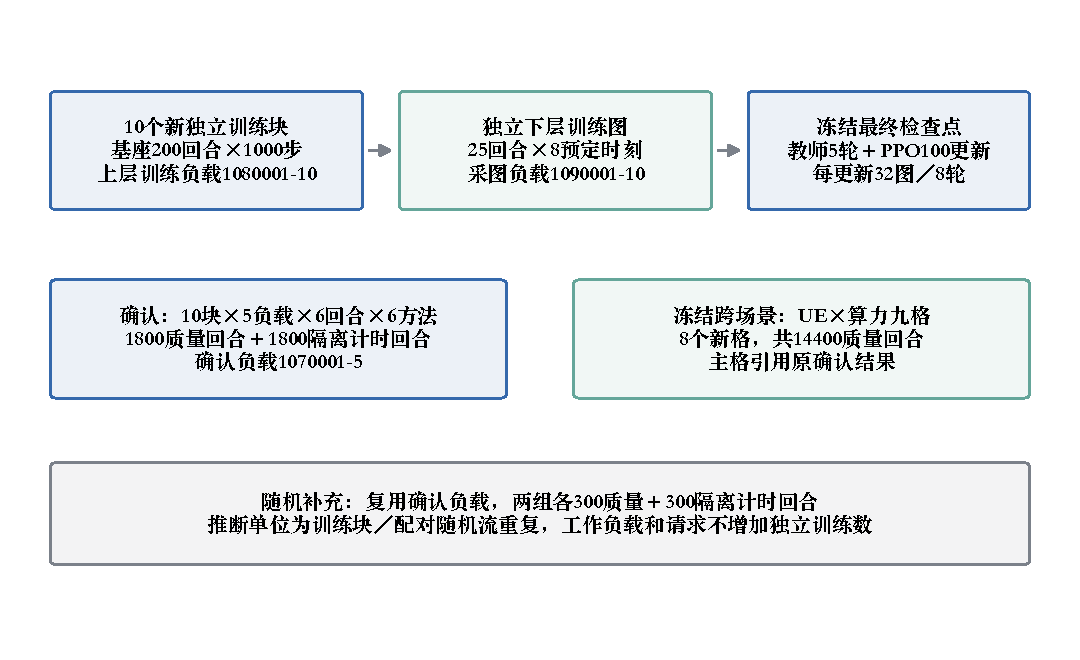
\includegraphics[width=0.98\textwidth]{../docs/figures/图5-4_训练确认数据划分}
 \bicaption{共同基座、下层训练图与独立确认的数据划分。图中回合是环境交互，配额 PPO 更新是固定训练图上的搜索训练}{Data split for shared foundations, lower-layer training graphs and independent confirmation}
 \label{legacy:fig:ch5-split}
\end{figure}

\subsection{即时教师与独立监督损失}

随机初始化的配额策略需要从大量无改善迁移和非法候选中学习，有限匹配预算下直接优化可能较难发现有用方向。本文先使用训练图上的即时改进教师提供可执行的动作示例。教师从同一共同保底和初始匹配出发，对当前有效迁移逐一尝试条件匹配，在合法且满足能耗上限的候选中选择优于当前目标的动作；没有找到即时改进时标记 STOP。教师总匹配预算为 $128$，包括初始匹配、试探候选和被选中迁移，不能把教师评价当作免费的真值查询。

教师标签是其实际找到的动作，并非穷举配额空间的全局最优标签。即时改进教师也不一定能发现需要先经过较差状态的多步路径；这一限制说明监督阶段的作用是提供初始搜索偏好，而不是替代后续强化学习。每条样本保存当时的当前/最好图、有效动作集合和教师动作。对样本集 $\mathcal D_{\mathrm T}$，监督损失为
\begin{equation}
 \mathcal L_{\mathrm{BC}}(\theta)=
 -\frac{1}{|\mathcal D_{\mathrm T}|}
 \sum_{(s,a^{\mathrm T})\in\mathcal D_{\mathrm T}}
 \log\pi_\theta(a^{\mathrm T}\mid s).
 \label{legacy:eq:ch5-bc-loss}
\end{equation}
监督预训练采用 $5$ 轮、小批量 $64$ 和梯度范数上限 $0.5$，动作概率在样本保存的合法域内归一化。教师样本仅用于监督初始化，随后 PPO 使用策略自身采样的动作、概率和优势更新。

监督初始化提供即时改进偏好，PPO 随后优化自身采样搜索轨迹的累计回报。允许经过较差的可行状态，使搜索能够探索多步迁移路径。其相对共享框架对照的服务增量在第~\ref{legacy:sec:ch5-mechanisms}~节评价。

\subsection{有限搜索轨迹的优势估计}

每次 PPO 更新前固定策略参数，从本块训练图抽取 $32$ 个实例，各采集一条至多 $16$ 次匹配的搜索轨迹。汇总该批轨迹后开始更新，保存搜索状态 $s_\ell$、动作 $a_\ell$、采样对数概率、价值估计 $V_\phi(s_\ell)$、奖励及终止标记。

令 $d_\ell^{\mathrm{end}}\in\{0,1\}$ 为搜索终止标记，优势估计采用 GAE\cite{schulman2015high}：
\begin{equation}
 \delta_\ell=r_\ell+\gamma(1-d_\ell^{\mathrm{end}})V_\phi(s_{\ell+1})-V_\phi(s_\ell),
 \qquad \gamma=1,
 \label{legacy:eq:ch5-search-td}
\end{equation}
\begin{equation}
 \widehat A_\ell=\delta_\ell+\gamma\lambda(1-d_\ell^{\mathrm{end}})\widehat A_{\ell+1},
 \qquad\lambda=0.95,\qquad
 \widehat R_\ell=\widehat A_\ell+V_\phi(s_\ell).
 \label{legacy:eq:ch5-search-gae}
\end{equation}
搜索终点下一状态价值取零，递推在每条图轨迹边界停止。$\gamma=1$ 对应最多十余步的有限预算求解，而不是无限时域控制；它保留式~\eqref{legacy:eq:ch5-reward-telescope} 中改善与调用开销的完整权衡。价值训练目标使用未标准化的 $\widehat R_\ell$，策略梯度使用本次采样记录内标准化的优势。

标准化写作
\begin{equation}
 \widetilde A_\ell=\frac{\widehat A_\ell-\overline A}
 {\max(\operatorname{std}(\widehat A),10^{-6})}.
 \label{legacy:eq:ch5-adv-normalization}
\end{equation}
若某批图没有有效搜索记录，则跳过参数更新而不是制造奖励或动作。不同图可以有不同请求数和搜索长度；填充处理的是图张量，不增加真实优势样本。请求数、搜索步或教师标签数也不能计为独立训练单位。

\subsection{裁剪策略目标与概率一致性}

配额 PPO 采用分类动作分布，其新旧策略概率比为
\begin{equation}
 \rho_\ell(\theta)=
 \exp\left[\log\pi_\theta(a_\ell\mid s_\ell)
          -\log\pi_{\mathrm{old}}(a_\ell\mid s_\ell)\right].
 \label{legacy:eq:ch5-search-ratio}
\end{equation}
裁剪目标沿用 PPO 的有限更新思想\cite{schulman2017proximal}：
\begin{equation}
 \mathcal L_{\mathrm{policy}}=-\mathbb E_\ell\left[
 \min\left(\rho_\ell\widetilde A_\ell,
 \operatorname{clip}(\rho_\ell,0.8,1.2)\widetilde A_\ell\right)\right]
 -0.005\,\mathbb E_\ell[\mathcal H(\pi_\theta(\cdot\mid s_\ell))].
 \label{legacy:eq:ch5-search-ppo}
\end{equation}
价值损失为
\begin{equation}
 \mathcal L_{\mathrm{value}}=
 \frac12\mathbb E_\ell\left[(V_\phi(s_\ell)-\widehat R_\ell)^2\right].
 \label{legacy:eq:ch5-search-value}
\end{equation}
共享图编码器与动作、价值头一起最小化两项之和，Adam 学习率为 $3\times10^{-4}$，每次采样执行 $8$ 个 epoch、小批量 $64$，总计 $100$ 次 PPO 更新，梯度范数裁剪为 $0.5$。最终确认使用第 $100$ 次更新后的最后检查点，没有从开发或确认曲线中挑选最高 DSR 时刻。

PPO 的概率一致性在带访问去重的搜索中尤为重要。同一个配额在轨迹前段可能未访问、后段已经访问；如果训练时重算访问集合，动作分布的归一化域会改变，概率比就不再对应原采样策略。本方法把采样时掩码和当前/最好图作为不可变记录保存，并在首次梯度更新前检验重算概率比接近 $1$。并行轨迹来自相同冻结参数，教师标签不进入这些记录，从而使比值检验具有清楚的含义。

\begin{table}[!htbp]
 \centering
 \bicaption{已确认配额策略的训练设置}{Training settings of the confirmed quota policy}
 \label{legacy:tab:ch5-learning-settings}
 \begin{tabular}{lrlr}
  \toprule
  参数 & 数值 & 参数 & 数值 \\
  \midrule
  隐藏宽度 & $128$ & 消息传递层数 & $2$ \\
  请求/边/节点维数 & $4/14/16$ & 动作数 & $91$ \\
  每块采图回合 & $25$ & 每块训练图数 & $200$ \\
  教师总匹配预算/图 & $128$ & 监督预训练轮数 & $5$ \\
  PPO 更新次数 & $100$ & 每更新采样图数 & $32$ \\
  PPO epoch & $8$ & 监督/PPO小批量 & $64$ \\
  学习率 & $3\times10^{-4}$ & 梯度范数上限 & $0.5$ \\
  PPO 裁剪范围 & $[0.8,1.2]$ & 熵系数 & $0.005$ \\
  折扣因子 & $1$ & GAE参数 & $0.95$ \\
  在线匹配调用上限 & $16$ & 普通修复候选上限 & $128$ \\
  \bottomrule
 \end{tabular}
\end{table}

\subsection{共同基座与交互、教师计算预算}

每个独立训练块先重新训练覆盖需求分层基座 $200$ 个回合，每回合 $1000$ 步。共同基座包含上层与请求级 MAPPO 下层的最后参数、优化器与约束状态；确认中的六种下层方法从同一个上层基座出发。配额下层再使用 $25$ 个回合采图及离线监督/PPO计算；适配请求级下层则在冻结上层后继续训练 $75$ 个回合，并恢复原优化器及 DSR、MBS 约束状态。冻结请求级下层组保留基座下层，贪心、启发式和强随机不进行额外模型训练。

另有 $50$ 个回合用于固定策略数据采集，各方法复用相应记录。共同基座交互、配额采图、下层适配、教师匹配与网络优化具有不同计算需求，分别计量。实验比较对应这些预定训练设置下的方法表现，未将环境交互步数相同等同于总训练计算相同。

图~\ref{legacy:fig:ch5-training} 分别展示共同基座的环境训练与配额策略的搜索训练。两阶段具有不同横轴和奖励定义，曲线描述各自优化过程；方法的服务效果由独立确认评价。

\begin{figure}[!htbp]
 \centering
 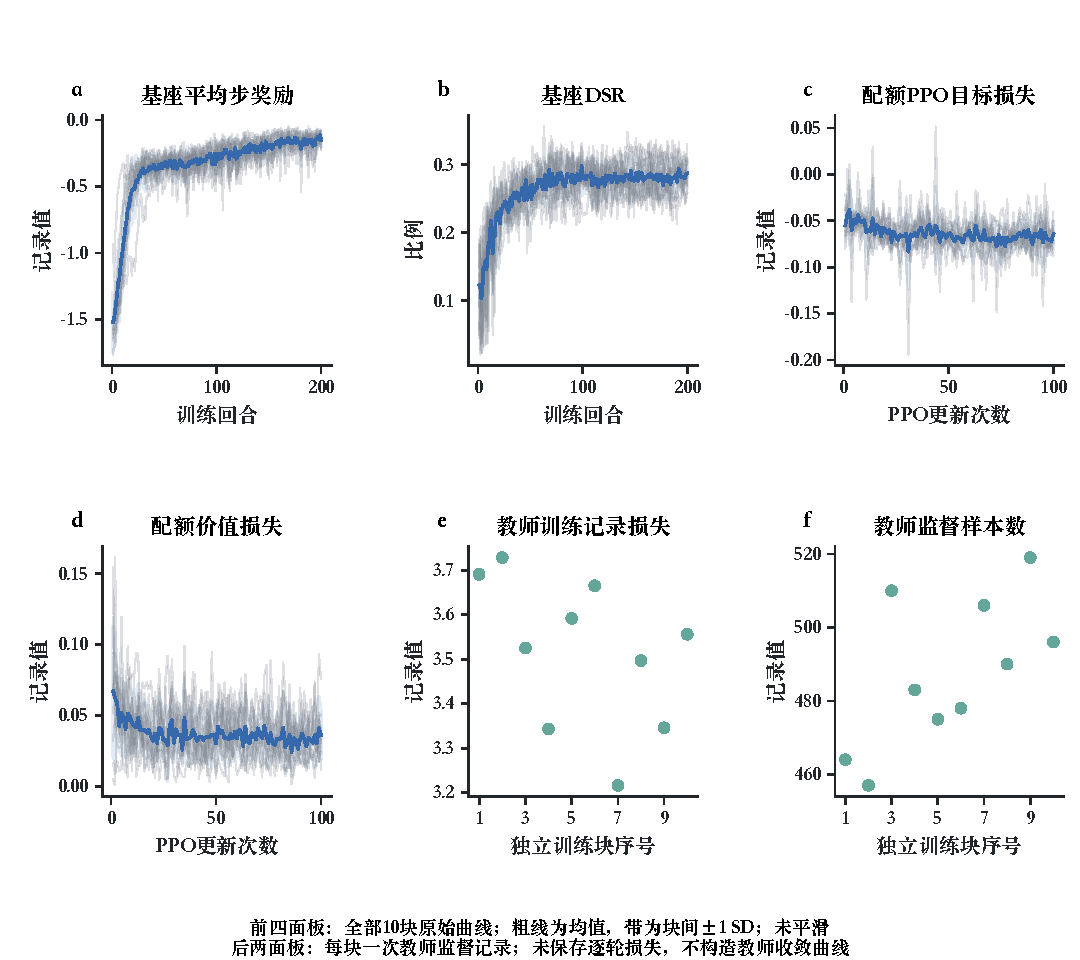
\includegraphics[width=0.98\textwidth]{../docs/figures/图5-5_基座与配额训练曲线}
 \bicaption{共同基座与配额策略的实际训练记录。前四面板依次为基座平均步奖励、基座DSR、配额PPO损失和价值损失：细线为十块原始曲线，粗线和带分别为块间均值与正负一个标准差；未平滑。后两面板为每块一次教师监督损失记录和样本数；未保存逐轮损失，故不绘制教师收敛曲线。环境回合、优化更新与训练块横轴分别对应不同阶段}{Actual training records of the foundation and quota policy; curves show ten blocks, and teacher panels show one recorded summary per block}
 \label{legacy:fig:ch5-training}
\end{figure}


\chapter{原十块确认、冻结九格及事后费用诊断}
\label{app:legacy-results}
本附录的SF-HLM均特指原学习配额变体。原主DSR不计调度等待；原十块与第五章新二十块属于不同方法、样本与费用协议，不合并统计。原九格仅检验原学习变体，不能替代解析主方法的跨负载及算力确认。末节事后费用评分保持原动作及状态，费用未回写环境。以下保留原数值和比较对象。

\section{独立确认设计与统计方法}
\label{legacy:sec:whole-protocol}
\label{legacy:sec:ch5-protocol}

\subsection{场景、种子分割与最后检查点}

主场景包含五架 UAV、一百 UE、一个 MBS 及 $700\,\mathrm{m}\times700\,\mathrm{m}$ 区域，通信、请求生成、能量动态、自然接纳和奖励设置保持一致。开发使用五个训练块，独立确认使用十个未参与模型选择的训练块，并区分基座、下层训练与确认负载。候选结构、模型选择规则、检验族和性能判据均在确认前确定。

\begin{table}[!htbp]
 \centering
 \bicaption{SF-HLM 独立确认的数据与模型分割}{Data and model split for independent SF-HLM confirmation}
 \label{legacy:tab:ch5-seeds}
 \begin{tabular}{lp{0.65\textwidth}}
  \toprule
  用途 & 固定设置 \\
  \midrule
  独立训练块 & $1060001$--$1060010$，共 $10$ 块 \\
  基座训练负载 & $1080001$--$1080010$，与各训练块一一对应 \\
  下层采图/适配负载 & $1090001$--$1090010$，与各训练块一一对应 \\
  配额下层初始化 & $1100001$--$1100010$，与各训练块一一对应 \\
  确认工作负载 & $1070001$--$1070005$，全部方法配对复用 \\
  评价长度 & 每块每负载 $6$ 回合，每回合 $1000$ 步 \\
  模型选择 & 基座训练与配额更新均固定最后检查点 \\
  六方法质量评价 & $6\times10\times5\times6=1800$ 回合 \\
  独立软件计时 & 另 $1800$ 回合，在预留物理核心重放同一策略 \\
  \bottomrule
 \end{tabular}
\end{table}

所有学习、贪心、启发式和强配额随机方法在同一训练块内复用共同上层参数，工作负载与初始外生流配对。不同卸载会改变后续能量、缓存和观测，因此即使上层参数相同，长期轨迹也可能分化；本章评价是闭环运行，不是冻结几何下的反事实分配。配对只要求潜在请求、外生随机序列和模型对应关系按协议一致，并不要求每个时隙状态或生成服务请求分母完全相同。

六种核心方法的质量评价覆盖 $180$ 万个环境步。软件计时重放相同模型与外生流，分配及真实物理计数与质量评价一致。两类运行分别用于服务质量统计和隔离时间测量，独立训练重复数保持十个。

\subsection{六个核心对照与两种补充随机策略}

表~\ref{legacy:tab:ch5-controls} 区分下层优化包与学习机制对照。启发式按当前合法目标的预测截止期风险选择配额迁移；强配额随机在有效迁移中随机选择，两者都拥有共同保底、条件匹配、最好保留和 $16$ 次调用上限。它们不能与“每请求随机选一个目标”混为同一种随机基线。

\begin{table}[!htbp]
 \centering
 \bicaption{完整下层与学习机制对照的组成}{Components of complete lower-layer and learning-mechanism controls}
 \label{legacy:tab:ch5-controls}
 \small
 \begin{tabularx}{\textwidth}{p{0.29\textwidth}Y}
  \toprule
  方法 & 下层与比较用途 \\
  \midrule
  学习配额搜索 & 二部图 PPO 选择配额迁移，条件匹配；SF-HLM \\
  启发式配额搜索 & 相同强框架与预算，按预测风险选择迁移；学习机制对照 \\
  强配额随机搜索 & 相同强框架与预算，在有效迁移中随机；严格学习增量对照 \\
  贪心＋普通修复 & 原始贪心后做最多 $128$ 次普通修复；主要实用对照 \\
  冻结请求级下层＋修复 & 基座请求级 MAPPO 提案后共同修复；主要学习对照 \\
  适配请求级下层＋修复 & 冻结上层后继续 $75$ 回合原下层训练，再共同修复 \\
  相同上层＋逐请求随机卸载 & 共同质量掩码内逐请求均匀随机；移除整个下层优化包 \\
  全随机（质量掩码内） & 二维轨迹在 $[-1,1]^2$ 独立均匀采样，卸载逐请求随机 \\
  \bottomrule
 \end{tabularx}
\end{table}

请求级 MAPPO 对照保留原始提案与采样概率，再以共同普通修复生成执行分配。适配组恢复基座优化器及自适应约束状态，继续训练已有下层；冻结组保持下层参数固定。两组均使用共同能耗参照和修复流程，与配额匹配组成完整方法对照。

确认后增加两种随机对照，复用十套固定模型和五个确认负载，每种方法运行 $300$ 个质量回合与 $300$ 个隔离计时回合。两者保持质量掩码、自然接纳和物理规则，移除贪心、普通修复、条件匹配、配额搜索、最好保留及预测能耗筛选。全随机评价完整系统，相同学习上层加逐请求随机卸载评价完整下层；学习搜索增量则由共享求解框架的强随机对照评价。

\subsection{请求计数聚合与十个独立统计单位}

令 $b=1,\ldots,10$ 为独立训练块，$w=1,\ldots,5$ 为工作负载，$e=1,\ldots,6$ 为评估回合，$t=1,\ldots,1000$ 为时隙。对方法 $a$，先合并同一块的全部请求计数：
\begin{equation}
 G_b^a=\sum_{w,e,t}G_{bwet}^a,\qquad
 A_b^a=\sum_{w,e,t}A_{bwet}^a,\qquad
 S_b^a=\sum_{w,e,t}S_{bwet}^a.
 \label{legacy:eq:ch5-block-counters}
\end{equation}
再定义块级指标
\begin{equation}
 D_b^a=\frac{S_b^a}{G_b^a},\qquad
 a_b^a=\frac{A_b^a}{G_b^a},\qquad
 q_b^a=\frac{S_b^a}{A_b^a},\qquad D_b^a=a_b^aq_b^a.
 \label{legacy:eq:ch5-block-metrics}
\end{equation}
主场景各块均有非零生成与接纳计数。空统计单元采用正分母保护，保持零成功计数。

方法的描述均值是 $\overline D^a=10^{-1}\sum_bD_b^a$。这使每个独立模型块的权重相同，不让生成请求稍多的块获得更大统计权重。它也不同于先求每回合比率再平均，因为后者会让请求较少的回合与请求较多的回合占相同权重。本文使用请求计数汇总的定义，并在表、图和差值检验中保持一致。

跨块均值一般不满足 $\overline D=\overline a\,\overline q$，其差为
\begin{equation}
 \overline D-\overline a\,\overline q
 =\frac1{10}\sum_{b=1}^{10}(a_b-\overline a)(q_b-\overline q).
 \label{legacy:eq:ch5-mean-product}
\end{equation}
接纳率与条件完成率的跨块均值用于描述方向，精确分解则按同块计数计算，以保留块间协变。

训练块是主推断单位。五工作负载和六回合改善块内估计，单个请求提供服务计数，都不扩充独立训练样本数。强随机搜索在每块对应同一个学习上层，并具有独立策略随机流，因此其变化包含共同模型和策略随机性。全随机没有训练过程，补充评价的十个块只是与十套模型配对的独立随机流重复，不应称作十个全随机训练种子。

\subsection{配对区间、多重比较与预定门槛}

候选 $a$ 与对手 $c$ 的块级差值为 $\Delta_b=D_b^a-D_b^c$。其均值、标准差与双侧 $95\%$ 配对 $t$ 区间为
\begin{equation}
 \overline\Delta=\frac1{10}\sum_b\Delta_b,\quad
 s_\Delta^2=\frac1{9}\sum_b(\Delta_b-\overline\Delta)^2,\quad
 \mathrm{CI}_{95}=\overline\Delta\pm t_{0.975,9}\frac{s_\Delta}{\sqrt{10}}.
 \label{legacy:eq:ch5-paired-ci}
\end{equation}
$t_{0.975,9}$ 约为 $2.262$，配对检验以十个训练块差值为数据。DSR 的绝对差异以百分点表示。

主检验族在确认前固定为学习相对贪心修复、冻结请求级下层修复和适配请求级下层修复三项。学习相对启发式与强随机属于独立的两项机制族。每族内部按 Holm 方法校正：将 $K$ 个原始双侧 $p$ 值升序排列，计算
\begin{equation}
 p_{(i)}^{\mathrm{Holm}}=
 \min\left\{1,\max_{h\le i}(K-h+1)p_{(h)}\right\}.
 \label{legacy:eq:ch5-holm}
\end{equation}
三个主性能比较、两个机制比较和两个补充随机比较分别组成检验族，按对应评价前确定的范围校正。

每个主比较须同时满足：DSR 均值增益至少 $1$ 个百分点、配对区间下界为正、Holm 校正 $p<0.05$、仿真环境记录的 UAV 总能耗的块级比值平均不超过 $1.05$，以及候选每块完整软件 p95 小于 $1\,\mathrm{s}$。能耗比定义为
\begin{equation}
 \overline\eta_{a/c}=\frac1{10}\sum_b\frac{E_b^a}{E_b^c}.
 \label{legacy:eq:ch5-energy-ratio}
\end{equation}
块级能耗比的平均值与两个总体能耗均值之比具有不同权重。预测能耗筛选约束单次分配，性能判据评价仿真机队总能耗；统计显著性与预定实用增益也分别报告。

学习与强随机的差值另进行精确符号翻转敏感性检验。十块配对差形成 $2^{10}$ 种符号组合，以均值绝对值检验零假设，考察小样本推断对分布假设的敏感性。该检验要求零假设下差值符号可交换，与配对 $t$ 推断并列报告。

\subsection{能耗、公平性、MBS 与完整软件计时}

仿真环境记录的总能耗 $E_b^a$ 汇总五架 UAV 的飞行与作业等全部环境记录，再除以块内 $30000$ 个时隙得到 J/步。该量不包括 MBS 计算、真实部署的新增控制通信和获取大范围需求信息的全部费用，所以 UAV 节能与全网节能是不同主张。公平性按第三章 Jain 指数逐时隙计算，再在块内平均；MBS 占比为块内送往 MBS 的请求数除以已接纳服务请求数。MBS 分母是接纳数，不是全部生成数。

主评价的请求时延包含模型规定的通信与计算路径，不计调度器求解等待。完整软件时间从移动前输入准备开始，包含观测构造、两层策略推理、共同保底、配额搜索、匹配、动作映射及逻辑消息编码，排除环境物理仿真和结果落盘。先在各训练块 $30000$ 次策略调用上计算 p95，再跨块平均；每块最大 p95 单独用于预定门槛。隔离计时在预留物理核心运行，与共享集群上的质量评估计时区分。相同模型和外生流重放保证时间测量不改变动作及质量，硬件和软件测量条件限制其可外推范围。

逻辑上传和下载字节由请求行、动作与摘要的序列化记录计算，用于描述协调信息规模。当前评价未将其转换为实际通信等待或能源开销。进一步研究可在请求截止期判定和能耗结算中加入上报、汇总及下发成本，独立评价通信受限条件下的服务质量。

\section{主场景性能与完整下层优化包的收益}
\label{legacy:sec:whole-results}
\label{legacy:sec:ch5-results}

\subsection{代表轨迹与实际注意力记录}

先以一个事先固定的评估实例展示集群在线运行形态：取首个确认训练块 $1060001$、首个工作负载 $1070001$、第 $0$ 回合，绘制学习配额与贪心修复的五机轨迹、实际航程和最小机间距，如图~\ref{legacy:fig:ch5-trajectories}。两方法起始外生条件和冻结上层参数相同，但下层执行影响电量、缓存和后续观测，轨迹随闭环状态演化可以不同。选择首实例而不是视觉上最有利的轨迹，有助于把运行示例与全样本性能推断分开。

\begin{figure}[!htbp]
 \centering
 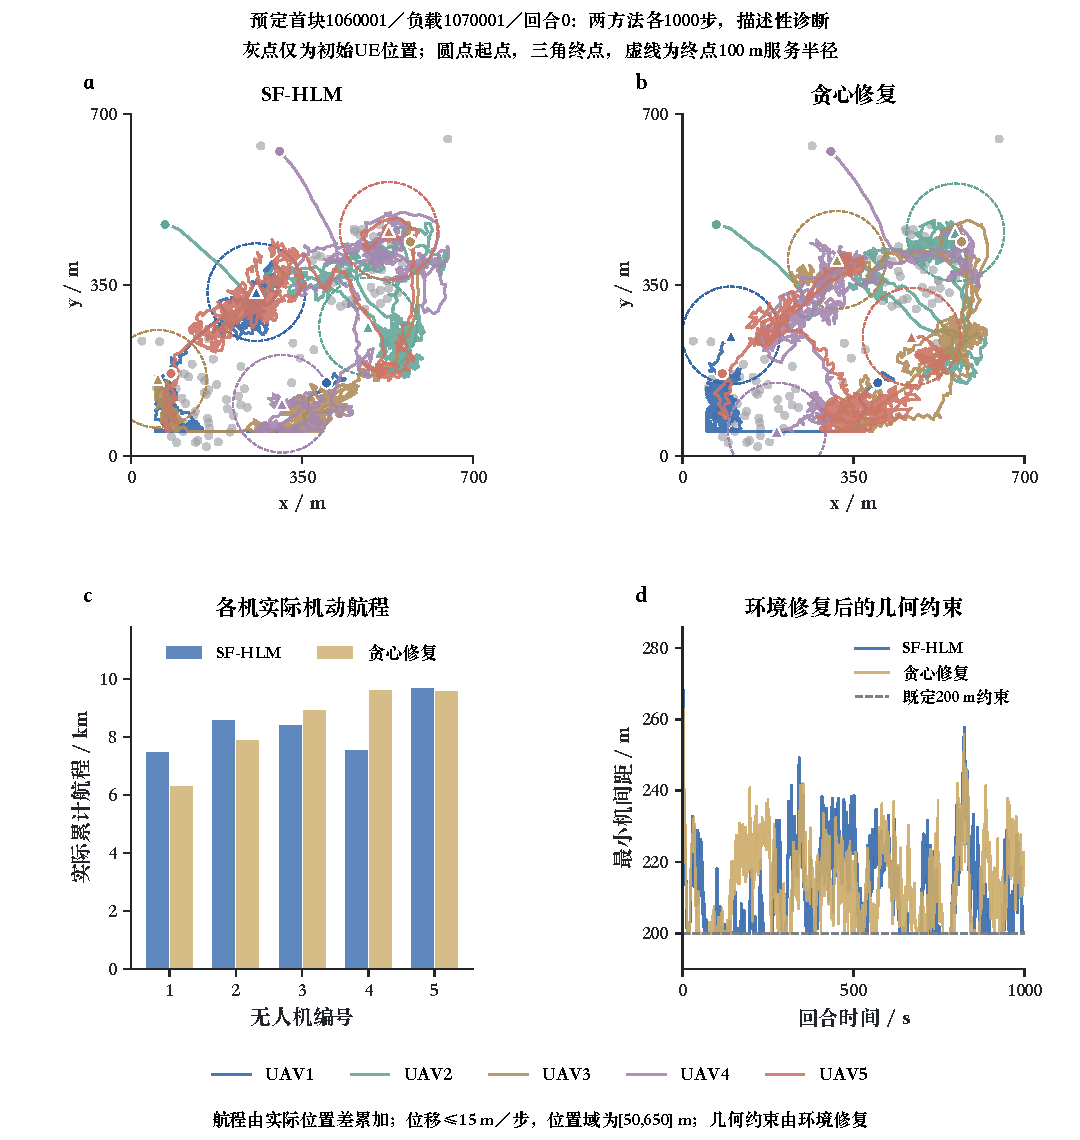
\includegraphics[width=0.98\textwidth]{../docs/figures/图5-6_UAV轨迹与覆盖}
 \bicaption{预选首确认回合的集群空间机动记录。上排为两方法五机轨迹，灰点仅表示初始 UE 位置，虚线为终点 $100\,\mathrm{m}$ 服务圆；下排为逐机实际水平航程与最小机间距。$200\,\mathrm{m}$ 间距线是既定几何约束；本图只描述各方法一个回合}{Swarm trajectories, per-UAV horizontal path lengths and minimum separation in one preselected episode per method; UE markers show initial positions only}
 \label{legacy:fig:ch5-trajectories}
\end{figure}

逐机航程由实际位置差累加，即 $\ell_u=\sum_{t=0}^{T-1}\|\mathbf q_u(t+1)-\mathbf q_u(t)\|_2$，其中 $T=1000$，$\ell_u$ 的单位为 m；它不使用网络原始动作模长代替执行位移。该回合中，SF-HLM 五机航程之和约为 $41.664\,\mathrm{km}$，贪心修复约为 $42.291\,\mathrm{km}$。这些数值描述预选实例的机动分工，不代表全评估总体中的航程差异。最小机间距按 $d_*(t)=\min_{u<v}\|\mathbf q_u(t)-\mathbf q_v(t)\|_2$ 逐步计算；两方法的实际位置记录连续，最大单步位移不超过 $15\,\mathrm{m}$，最小间距为 $200\,\mathrm{m}$，核验采用 $10^{-6}\,\mathrm{m}$ 浮点容差。该结果检查的是修复后的离散位置，而不是学习策略独立提供的连续飞行避碰能力。

轨迹图的地面散点表示初始 UE 位置，服务圆表示终点几何，动态接纳率由完整请求计数计算。图~\ref{legacy:fig:ch5-actual-attention} 展示同一回合第 $500$ 步上层 Actor 的注意力，采用该步输入、模型权重与实际前向缩放、掩码，描述可见邻机和需求的信息聚合。

\begin{figure}[!htbp]
 \centering
 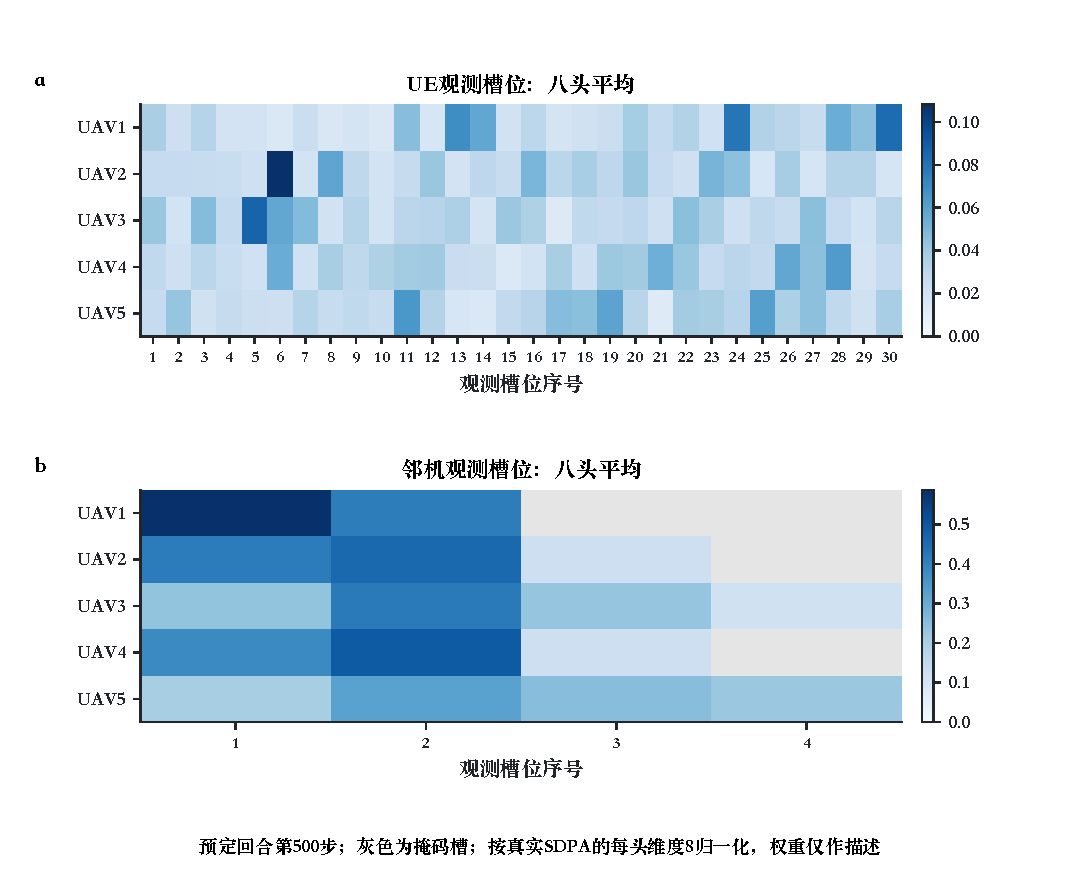
\includegraphics[width=0.98\textwidth]{../docs/figures/图5-7_实际前向注意力}
 \bicaption{代表确认回合第 $500$ 步上层 Actor 的实际前向注意力记录。权重说明该状态下的信息聚合，不作为注意力贡献的独立因果证明}{Actual upper-Actor attention at step 500 of the representative episode; a descriptive forward-pass diagnostic}
 \label{legacy:fig:ch5-actual-attention}
\end{figure}

注意力图描述代表状态的信息聚合，独立评价则检验完整策略的服务效果。核心六组共享需求感知上层，因此本章比较集中于同一轨迹基座上的下层任务组织，上层观测及结构比较见第三章。

\subsection{八种方法的截止期满足表现}

表~\ref{legacy:tab:ch5-main-quality} 和图~\ref{legacy:fig:ch5-eight-dsr} 汇总六种核心方法的独立确认与两种补充随机评价。补充对照复用相同模型和确认负载，均以实际生成服务请求为分母并按块汇总计数。SF-HLM 的 DSR 为 $34.244\%$，在八种方法中具有最高描述均值。以下差值均来自本章对应的配对评价。

\begin{table}[!htbp]
 \centering
 \bicaption[原十块主场景服务指标]{一百 UE 主场景的服务指标（先合并块内请求计数，再跨块平均）}{Service metrics in the 100-UE setting, obtained from within-block request counts and between-block averaging}
 \label{legacy:tab:ch5-main-quality}
 \begin{tabular}{lrrr}
  \toprule
  方法 & DSR/\% & 接纳率/\% & 接纳后完成率/\% \\
  \midrule
  学习配额搜索 & \textbf{34.244} & 57.339 & 59.819 \\
  启发式配额搜索 & 33.475 & 57.342 & 58.472 \\
  强配额随机搜索 & 34.100 & 57.379 & 59.517 \\
  贪心＋普通修复 & 32.821 & 57.367 & 57.305 \\
  冻结请求级下层＋修复 & 32.236 & 57.375 & 56.309 \\
  适配请求级下层＋修复 & 32.052 & 57.383 & 55.953 \\
  \midrule
  全随机（质量掩码内） & 15.428 & 33.797 & 45.673 \\
  相同上层＋逐请求随机卸载 & 23.640 & 57.431 & 41.222 \\
  \bottomrule
 \end{tabular}
\end{table}

\begin{figure}[!htbp]
 \centering
 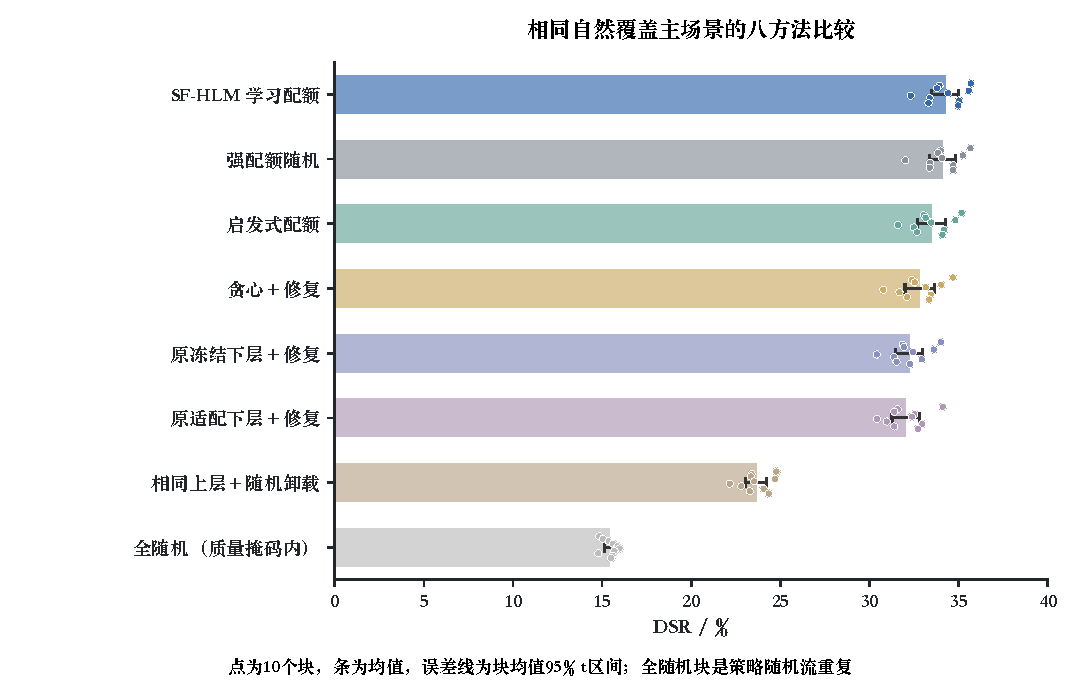
\includegraphics[width=0.97\textwidth]{../docs/figures/图5-8_八方法DSR比较}
 \bicaption{主场景八种方法的 DSR 比较。六种核心方法与两种补充随机对照分别标识；统计单位为十个模型或随机流配对块}{DSR comparison of eight methods in the main setting, with core and supplementary controls identified; ten paired model or random-stream blocks}
 \label{legacy:fig:ch5-eight-dsr}
\end{figure}

学习相对贪心修复的主增益为 $1.423$ 个百分点，相对冻结请求级下层、适配请求级下层修复分别为 $2.008$ 和 $2.192$ 个百分点，完整区间与校正检验列于表~\ref{legacy:tab:ch5-primary}. 三项差值均在十个训练块上同向为正；图~\ref{legacy:fig:ch5-primary-blocks} 展示这些块级配对差，说明均值优势并非由单个异常训练块独自支撑。三项均达到预定 $1$ 个百分点实用目标，区间下界为正，并通过三比较 Holm 校正。

\begin{table}[!htbp]
 \centering
 \bicaption[原三主对照的DSR差与能耗比]{三个预定主对照的配对 DSR 差值与仿真环境记录的 UAV 能耗比}{Paired DSR effects and simulated UAV energy ratios for the three prespecified primary controls}
 \label{legacy:tab:ch5-primary}
 \small
 \begin{tabular}{lrrrr}
  \toprule
  学习减对手 & 差值/百分点 & $95\%$区间/百分点 & Holm $p$ & 能耗比 \\
  \midrule
  贪心＋普通修复 & $+1.423$ & $[1.258,1.587]$ & $2.22\times10^{-8}$ & $0.9094$ \\
  冻结请求级下层＋修复 & $+2.008$ & $[1.808,2.208]$ & $8.92\times10^{-9}$ & $0.9656$ \\
  适配请求级下层＋修复 & $+2.192$ & $[1.903,2.481]$ & $3.46\times10^{-8}$ & $0.9803$ \\
  \bottomrule
 \end{tabular}
\end{table}

\begin{figure}[!htbp]
 \centering
 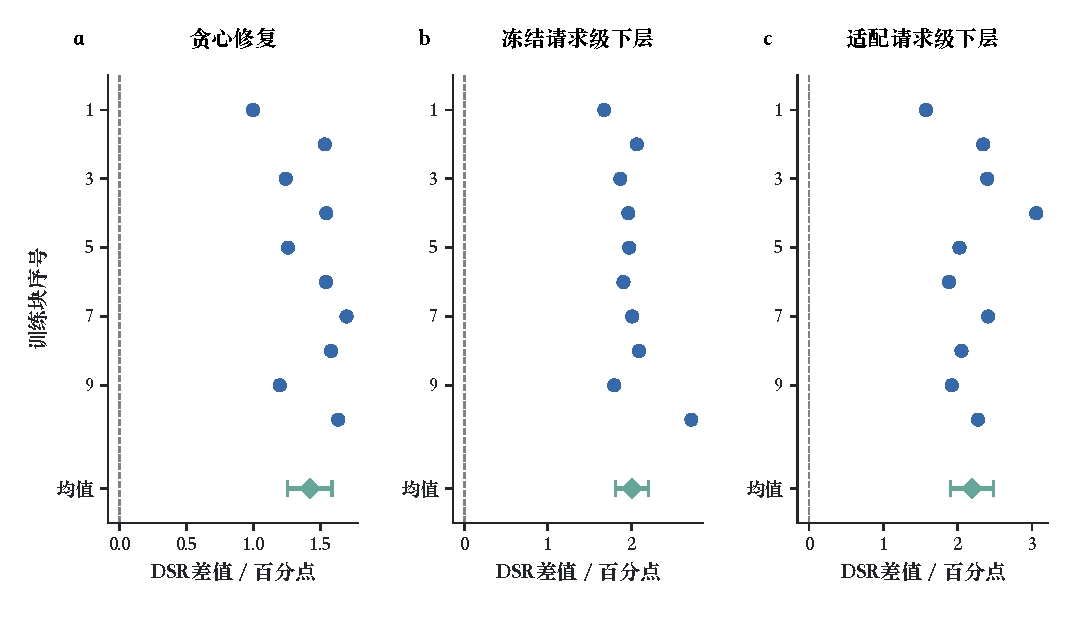
\includegraphics[width=0.97\textwidth]{../docs/figures/图5-9_主比较训练块配对差}
 \bicaption{SF-HLM 相对三个主对手的十训练块配对差。每个块先合并五工作负载、六回合的请求计数}{Per-training-block DSR differences against the three primary controls, based on pooled requests within each block}
 \label{legacy:fig:ch5-primary-blocks}
\end{figure}

两种请求级学习对照使用共同普通修复，适配组另继续训练下层。在一百 UE 主场景、十个独立训练块及预定训练设置下，三个主比较支持 SF-HLM 完整下层的端到端 DSR 改善。教师计算和不同训练流程分别记录，结构贡献由后续共享框架机制对照评价。

\subsection{接纳与接纳后质量的请求计数分解}

核心六方法的平均接纳率均约为 $57.3\%$。SF-HLM 与贪心的接纳率分别为 $57.339\%$ 和 $57.367\%$，接纳后完成率为 $59.819\%$ 和 $57.305\%$。共享上层下，改善主要体现为已接纳请求的执行质量；各方法仍按自身闭环轨迹统计请求，保留状态分化的影响。

图~\ref{legacy:fig:ch5-outcomes} 将生成请求分为未接纳、接纳后超时与按时完成三个互斥部分。块内占比分别为 $(G-A)/G$、$(A-S)/G$ 和 $S/G$，相加为 $1$；跨块平均保持该线性恒等式。SF-HLM 中三个部分约为 $42.661\%$、$23.095\%$ 和 $34.244\%$。同上层逐请求随机卸载的按时完成率仅为 $41.222\%$，而接纳率仍为 $57.431\%$，显示进入服务范围后的执行质量构成主要差距。

\begin{figure}[!htbp]
 \centering
 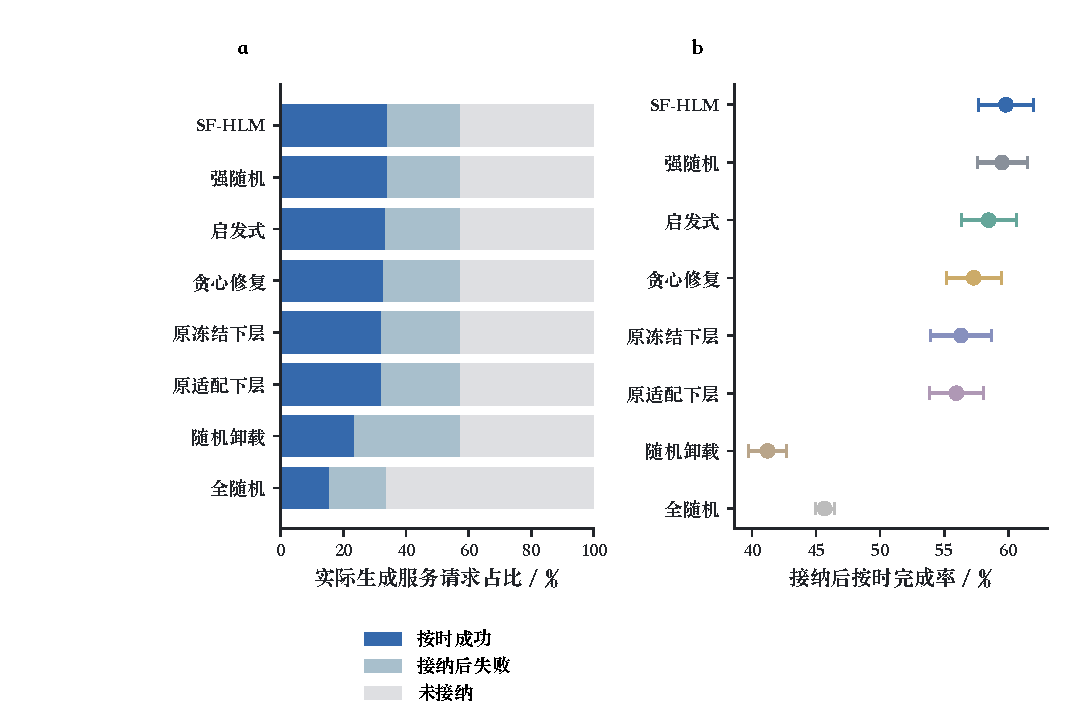
\includegraphics[width=0.98\textwidth]{../docs/figures/图5-10_请求结果与接纳后质量}
 \bicaption{生成请求的互斥结果分解与接纳后完成率。三种结果按同块计数计算后平均，条件完成率以接纳请求为分母}{Mutually exclusive request outcomes and deadline completion conditional on admission}
 \label{legacy:fig:ch5-outcomes}
\end{figure}

全随机接纳率为 $33.797\%$，明显低于采用学习上层的策略组，反映完整系统在形成服务机会方面的收益。保留学习上层之后，随机卸载的接纳后质量仍远低于配额匹配。这两个对照有助于解释覆盖与服务质量各自的作用，但不是固定状态下可相加的因果分解：全随机改变运动，随机卸载改变能量和后续观测，二者的状态轨迹不同。本文使用分解描述实际结果，不把 $18.816$ 个百分点机械拆成几个独立组件贡献。

\subsection{UAV 能耗与 MBS 依赖}

表~\ref{legacy:tab:ch5-main-cost} 和图~\ref{legacy:fig:ch5-energy-mbs} 同时报告 UAV 机队能耗与 MBS 占比。SF-HLM 的仿真环境记录的 UAV 能耗为 $30394.4\,\mathrm{J}/\text{步}$，低于贪心修复的 $33419.9\,\mathrm{J}/\text{步}$；按块能耗比平均计，降低约 $9.06\%$。相对冻结与适配请求级下层修复，块级能耗比为 $0.9656$ 与 $0.9803$。因此三个主比较的 DSR 改善没有以超过预定机队能耗门槛为代价。

\begin{table}[!htbp]
 \centering
 \bicaption{主场景 UAV 资源代价、公平性和完整软件时间}{UAV resource costs, fairness and full-policy software timing in the main setting}
 \label{legacy:tab:ch5-main-cost}
 \small
 \begin{tabular}{lrrrr}
  \toprule
  方法 & UAV能耗/(J/步) & MBS占比/\% & 公平性 & 块p95均值/ms \\
  \midrule
  学习配额搜索 & $30394.4$ & $9.83$ & $0.9239$ & $109.24$ \\
  启发式配额搜索 & $31854.7$ & $2.42$ & $0.9209$ & $78.16$ \\
  强配额随机搜索 & $30123.1$ & $8.17$ & $0.9216$ & $73.47$ \\
  贪心＋普通修复 & $33419.9$ & $2.92$ & $0.9212$ & $17.59$ \\
  冻结请求级下层＋修复 & $31484.7$ & $3.07$ & $0.9207$ & $17.19$ \\
  适配请求级下层＋修复 & $31010.1$ & $4.14$ & $0.9208$ & $17.17$ \\
  全随机（质量掩码内） & $59649.6$ & $29.65$ & $0.7874$ & $4.70$ \\
  相同上层＋随机卸载 & $57503.7$ & $29.45$ & $0.9208$ & $6.57$ \\
  \bottomrule
 \end{tabular}
\end{table}

\begin{figure}[!htbp]
 \centering
 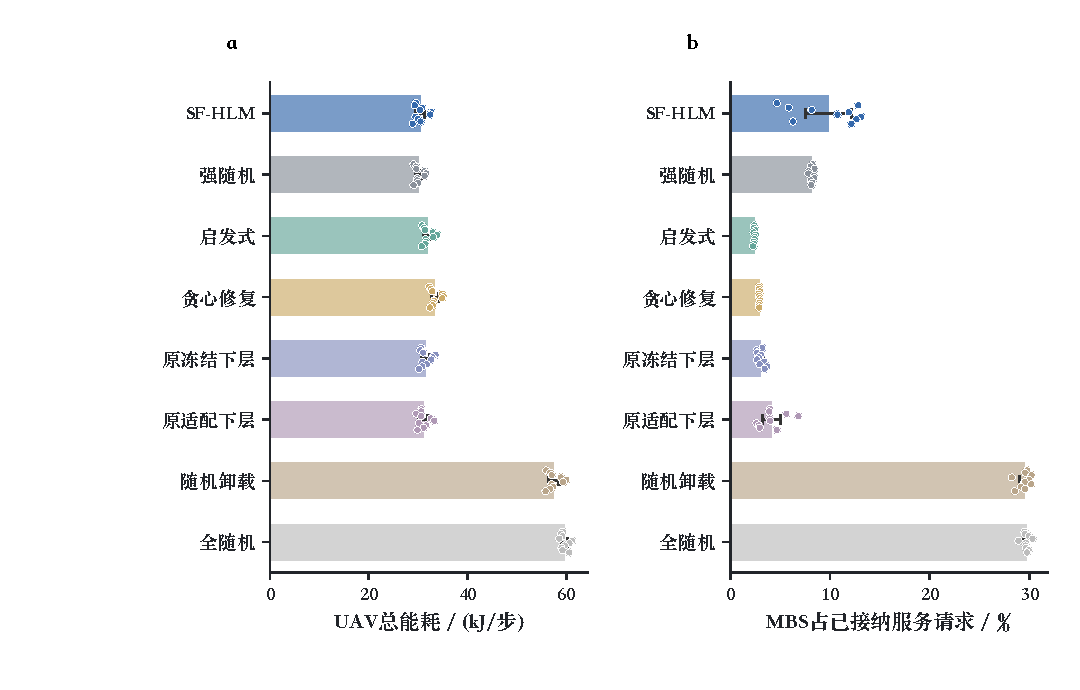
\includegraphics[width=0.98\textwidth]{../docs/figures/图5-11_UAV能耗与MBS依赖}
 \bicaption{仿真环境记录的 UAV 机队能耗与 MBS 依赖。图中能耗为 kJ/步，MBS 比例为 MBS 请求数除以接纳请求数；未计 MBS 全网费用}{Simulated UAV fleet energy in kJ per step and MBS fraction among admitted requests, excluding whole-network MBS costs}
 \label{legacy:fig:ch5-energy-mbs}
\end{figure}

SF-HLM 送往 MBS 的接纳请求比例为 $9.83\%$，高于贪心的 $2.92\%$ 和启发式的 $2.42\%$。在 MBS 单请求算力不共享的设置下，任务转移释放 UAV 算力并改变其计算与转发能耗。因此，UAV 能耗下降需结合 MBS 依赖解释，其统计范围未包含地面计算和完整网络能源。

逐请求随机卸载的 MBS 占比接近 $29.5\%$，却同时具有较低 DSR 和较高 UAV 能耗，说明 MBS 比例本身不是充分的性能解释。请求身份、回传路径、UAV 剩余批量和质量掩码共同影响结果。后续共同 MBS 数量快照诊断将进一步控制这一维度，检验配额匹配在固定 MBS 使用数量时仍有多少单步质量余量。

\begin{table}[!htbp]
 \centering
 \bicaption{主场景仿真机队能耗构成（每步及等权块占比）}{Simulated fleet energy components per step and equal-block shares}
 \label{legacy:tab:ch5-energy-components}
 \small
 \setlength{\tabcolsep}{4pt}
 \begin{tabular}{lrrrrrr}
  \toprule
  分项 & 学习/J & 占比/\% & 强随机/J & 占比/\% & 贪心/J & 占比/\% \\
  \midrule
  计算 & 29205.1 & 96.079 & 28934.0 & 96.048 & 32232.6 & 96.442 \\
  飞行与悬停 & 1166.4 & 3.846 & 1166.7 & 3.878 & 1166.9 & 3.496 \\
  服务通信 & 2.3 & 0.008 & 2.3 & 0.008 & 2.3 & 0.007 \\
  回源或回传 & 3.4 & 0.011 & 2.9 & 0.010 & 1.0 & 0.003 \\
  内容服务 & 16.8 & 0.055 & 16.8 & 0.056 & 16.8 & 0.050 \\
  WPT & 0.4 & 0.001 & 0.4 & 0.001 & 0.4 & 0.001 \\
  \midrule
  总计 & 30394.4 & 100.000 & 30123.1 & 100.000 & 33419.9 & 100.000 \\
  \bottomrule
 \end{tabular}
\end{table}

表~\ref{legacy:tab:ch5-energy-components} 使用原确认记录的逐步能耗分项，重放仅补充核验。先在每块合并六回合与五负载，再对十块等权平均；分项占比按各块分项除以该块总能耗后平均。分配因果能耗与上述分项有重叠，故不另加一项。计算项占三方法总费用约 $96\%$，说明本模型的节能排序主要受等效计算能耗影响。各项在未舍入时精确加总，总额复现原表；显示精度下的细小差异来自舍入。该模型分解不对应实测机载功率或续航。

\subsection{公平性、计算费用与可执行性}

SF-HLM公平性均值为 $0.9239$，核心六方法约在 $0.9207$ 至 $0.9239$ 范围；全随机为 $0.7874$。图~\ref{legacy:fig:ch5-fairness-time} 展示公平性和隔离软件 p95。SF-HLM 在共享上层组中保持较高的描述公平性，同时完整软件 p95 的块均值为 $109.24\,\mathrm{ms}$，各块为约 $103$--$114\,\mathrm{ms}$，最大为 $114.343\,\mathrm{ms}$，均小于预定 $1\,\mathrm{s}$ 阈值。该结果证明在本次隔离测量条件下，完整在线调用满足协议时间门槛。

\begin{figure}[!htbp]
 \centering
 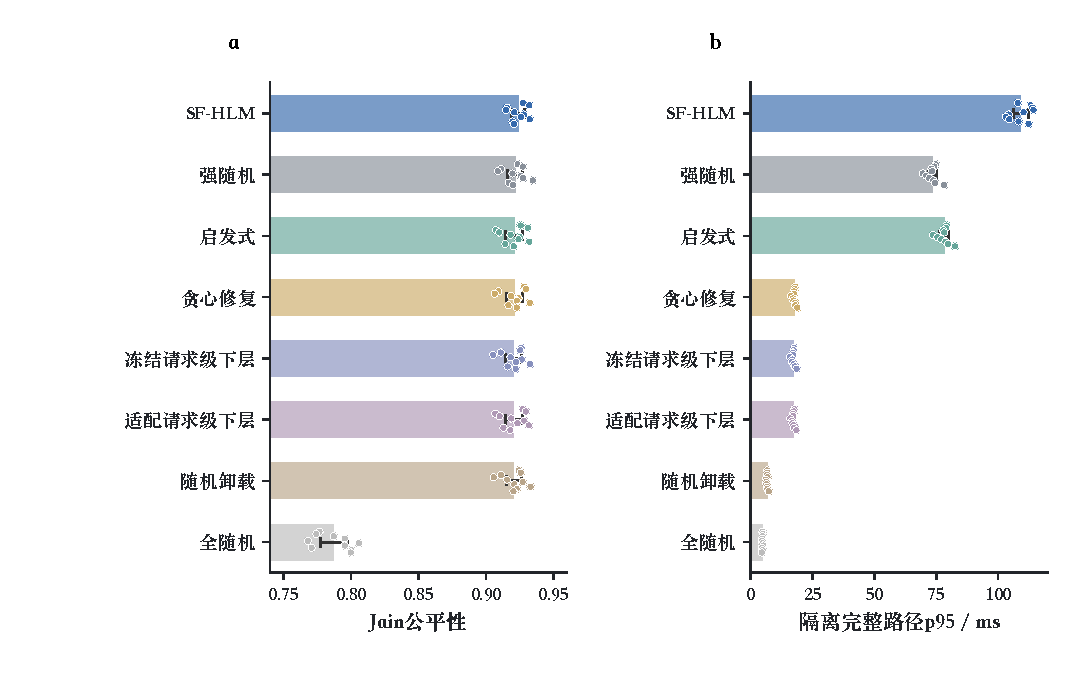
\includegraphics[width=0.98\textwidth]{../docs/figures/图5-12_公平性与隔离软件耗时}
 \bicaption{块级公平性与隔离完整软件 p95。p95先在每块全部调用上计算，再展示十块分布及其均值}{Block-level fairness and isolated full-policy p95, computed within each block before summarizing}
 \label{legacy:fig:ch5-fairness-time}
\end{figure}

SF-HLM 的完整时间高于强配额随机的 $73.47\,\mathrm{ms}$、启发式的 $78.16\,\mathrm{ms}$ 和贪心修复的 $17.59\,\mathrm{ms}$。图推理减少部分匹配尝试，同时增加网络前向费用。服务质量、公平性、匹配调用和全路径时间共同刻画方法收益与执行负担。

上述时间结论适用于规定服务器的隔离测量，未计入现实网络等待、MBS 排队及额外需求感知成本。当前服务指标与软件费用分别评价；满足一秒软件门槛不能直接证明计入求解等待后的截止期增益。面向机载部署仍需补充对应硬件与通信测量。

\section{完整框架与学习机制的分层解释}
\label{legacy:sec:ch5-mechanisms}

\subsection{完整系统与完整下层优化包}

补充随机评价显示，SF-HLM相对全随机 DSR 高 $18.816$ 个百分点，$95\%$ 配对区间为 $[17.840,19.791]$；相对相同上层逐请求随机卸载高 $10.604$ 个百分点，区间为 $[10.376,10.832]$。两项十块均为正，新两比较 Holm 校正通过，精确符号翻转 $p=0.001953$。对应仿真环境记录的 UAV 能耗块级比为 $0.5095$ 与 $0.5284$，即平均分别降低约 $49.0\%$ 和 $47.2\%$。

在共同质量合法域下，SF-HLM 使用贪心初始化、普通修复、预测能耗筛选、条件指派和最好保留，相对逐请求随机的 $10.604$ 个百分点改善评价这一完整优化框架。该结果显示，配额分解与条件匹配能够更有效地利用已形成的服务机会；学习策略在共享框架上的额外作用由下文机制对照进一步评价。

全随机的十个块对应独立随机动作流，与十套学习基座配对。补充评价复用模型与确认负载，区间反映这些条件下的模型和随机策略变化，不增加主确认的独立训练重复数。

\subsection{相同强框架上的学习配额增量}

共享强框架中，启发式 DSR 为 $33.475\%$，强配额随机为 $34.100\%$，学习为 $34.244\%$。学习相对启发式差 $0.769$ 个百分点，$95\%$ 区间 $[0.670,0.868]$，机制族 Holm $p=5.56\times10^{-8}$。这说明按图状态学习的配额选择优于本实验采用的风险排序启发式。该判断限定于所定义的启发式，不把一个启发式的结果外推为所有手工搜索规则都不能达到同样质量。

图~\ref{legacy:fig:ch5-mechanism-blocks} 展示共享框架的块级差。学习相对强随机增量为 $0.143$ 个百分点，区间 $[0.006,0.281]$；十块中六块为正，预定机制族 Holm $p=0.0422$。精确符号翻转检验则为 $p\approx0.0605$。小效应的两种推断存在差异，表明学习增量对统计方法具有敏感性。

\begin{figure}[!htbp]
 \centering
 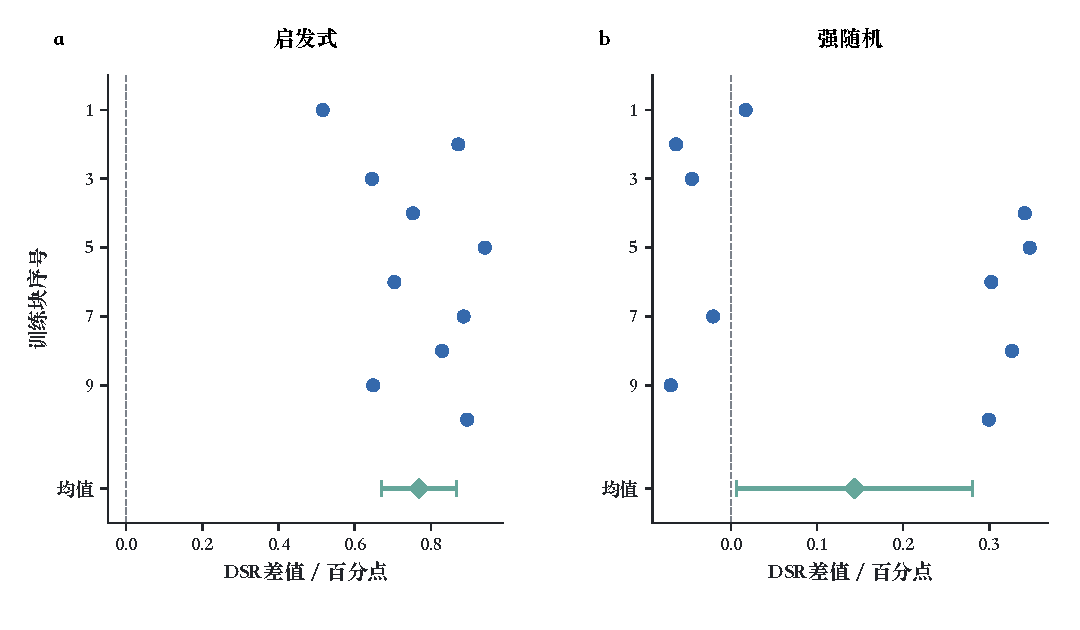
\includegraphics[width=0.97\textwidth]{../docs/figures/图5-13_强框架机制配对差}
 \bicaption{学习相对启发式和强配额随机的机制差。强随机共享初始化、修复、匹配、最好保留和相同调用预算}{Mechanism differences against heuristic and strong random quota search sharing the same optimization framework}
 \label{legacy:fig:ch5-mechanism-blocks}
\end{figure}

强随机在相同预算内接近学习质量，显示条件匹配、共同保底和最好保留发挥了较大作用。学习的额外收益较小，软件时间更长，相对强随机的 UAV 能耗块级比为 $1.0089$。因此，完整方法相对贪心与请求级学习修复的改善，以及共享框架上的学习增量，分别构成两个层次的结论。

\subsection{预测误差与实际服务验证}

SF-HLM每步预测超时数减实际接纳后超时数的均值为 $-0.304$ 个请求，平均绝对误差为 $0.366$；贪心相应值约为 $-0.209$ 和 $0.321$。负偏差说明观测预测总体上略低估真实超时，可能涉及缓存信念与真实状态的差别及执行细节。本文没有把预测器视为真实时延保证，所有 DSR 结果均由仿真环境的按时完成计数计算。

误差统计与条件最优证明并不矛盾。指派在给定预测量下精确优化，描述的是求解结构；预测量与实际执行之间仍存在误差，描述的是模型真实性。二者需要分别检查。如果只报告预测超时减少，可能把更乐观的预测当成性能提高；本章逐步重放实际计数，并在固定快照诊断中通过独立环境副本评价实际结果，使搜索时没有接触的执行真值用于最终验证。

\subsection{固定潜在服务请求分母复核}

相同外生随机流下，低电量 UE 会将潜在服务请求改为能量请求，因此实际生成服务请求分母有轻微策略依赖性。六个核心方法在全部确认回合中的潜在服务请求总数均为 $11397280$。保持原成功数不变，以共同潜在请求为分母，学习 DSR 均值为 $34.235\%$，强配额随机为 $34.091\%$；学习相对贪心的增益为 $1.421$ 个百分点，与预定实际分母下 $1.423$ 的方向和量级一致。

共同潜在分母复核仍保留三个主比较的增益，说明轻微实际分母变化不足以解释服务改善。该分析仅重新计算比率，保留原运行成功数和请求生成过程，作为实际分母 DSR 的敏感性结果。

\subsection{教师初始化与 PPO 的开发证据}
\label{legacy:sec:ch5-bc-ppo-development}

学习策略的独立确认比较教师初始化后经 PPO 更新的完整策略与共享求解框架对照，不能单独识别 PPO 更新的作用。为解释训练选择，补充五个历史训练块上的开发比较。该批次复用历史上层、训练图和开发负载，分别评价即时改进教师、多步路径教师及多步教师加动作效果特征的 BC 与 PPO 检查点。表~\ref{legacy:tab:ch5-bc-ppo-development} 报告各自 PPO 减 BC 的结果，不能与十块确认当作同一次重复实验合并。

\begin{table}[!htbp]
 \centering
 \bicaption{五训练块开发评价中的 PPO 相对 BC 差值}{PPO-minus-BC effects in the five-block development evaluation}
 \label{legacy:tab:ch5-bc-ppo-development}
 \small
 \begin{tabular}{lrrr}
  \toprule
  教师与输入配置 & DSR差/百分点 & 逐项95\%区间/百分点 & 正向块数 \\
  \midrule
  原即时改进教师 & $+0.935$ & $[+0.296,+1.573]$ & $5/5$ \\
  多步路径教师 & $-0.008$ & $[-0.704,+0.689]$ & $2/5$ \\
  多步教师＋动作效果特征 & $-0.364$ & $[-0.564,-0.164]$ & $0/5$ \\
  \bottomrule
 \end{tabular}
\end{table}

原教师配置下的开发差值与 PPO 有益的解释一致，但另外两种配置没有同样方向，说明强化学习更新的效果依赖教师、输入和搜索分布。仅五块时，前后两项精确符号翻转 $p$ 均为 $0.0625$，这些开发结果只用于方法选择解释，不替换主确认或升级为新的确证。当前学习策略的主要服务收益仍建立在共同修复、条件匹配和最好方案保留之上；是否采用学习搜索需要同时判断其批次质量增量与软件费用。其取舍结合第~\ref{legacy:sec:ch5-delay-audit}~节的截止期余量分析，不能仅凭开发阶段增量决定在线方法。

\section{冻结策略的负载与算力稳健性}
\label{legacy:sec:ch5-robustness}

\subsection{九格设置与冻结评价}

独立确认完成后，冻结十套基座和配额最后检查点，在 $60/100/140$ UE 与 $0.6/1.0/1.4$ 倍 UAV 算力的九格上评价。每格保持原五负载、六回合和六种核心方法，主格直接引用原 $1800$ 回合，八个新格共完成 $14400$ 个质量回合。权重、优化器、奖励、MBS 算力与自然接纳保持不变，只按协议调整 UE 数和 UAV 算力。这是固定策略面对新负载与资源规模的复验，不是各格重新训练后的场景适应比较。

上层保持训练时的 $30$ 个 UE 槽，超过容量的需求按相同排序截取。图下层按实际请求数构图，请求级 MLP 下层沿用填充与分块推理，均保持训练后的网络尺寸和权重。各方法使用相同变体环境，复用原训练块与确认负载，评价整套固定策略在规定格点上的表现。

\begin{table}[!htbp]
 \centering
 \bicaption{学习配额SF-HLM 在九格冻结评价中的 DSR}{DSR of the learned quota method across the nine frozen-policy settings}
 \label{legacy:tab:ch5-nine-grid}
 \begin{tabular}{lrrr}
  \toprule
  UE 数量 & $0.6$倍算力/\% & $1.0$倍算力/\% & $1.4$倍算力/\% \\
  \midrule
  $60$ & $44.430$ & $48.961$ & $50.746$ \\
  $100$ & $29.736$ & $34.244$ & $36.349$ \\
  $140$ & $22.142$ & $26.259$ & $28.263$ \\
  \bottomrule
 \end{tabular}
\end{table}

\begin{figure}[!htbp]
 \centering
 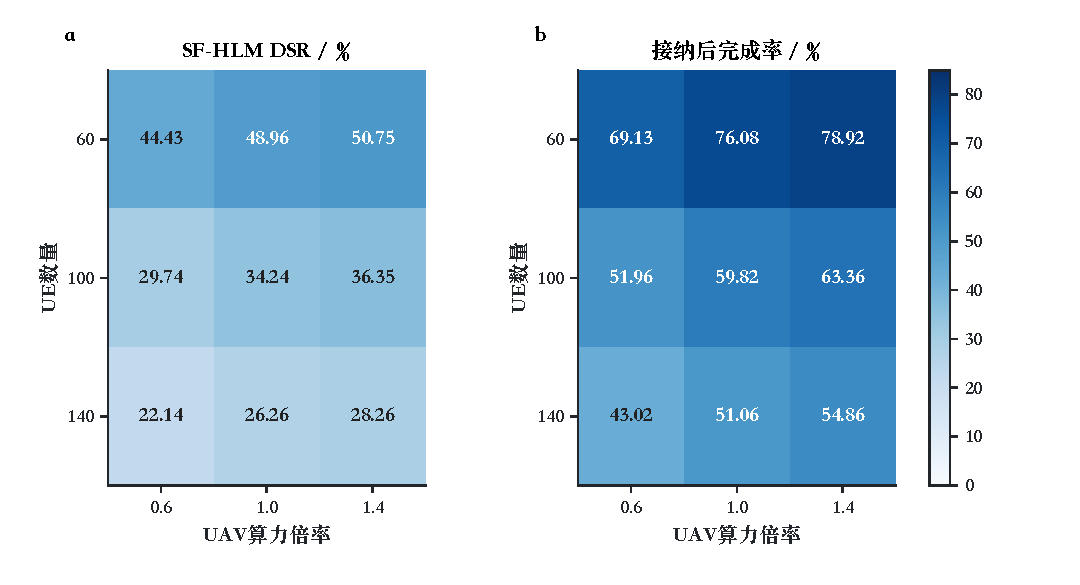
\includegraphics[width=0.98\textwidth]{../docs/figures/图5-14_九格冻结策略DSR}
 \bicaption{SF-HLM 冻结策略在 UE 数量与 UAV 算力九格中的 DSR（左）和接纳后按时完成率（右）。主格引用独立确认，其他格不重新训练；数值为十块均值}{DSR and conditional completion rate of the frozen SF-HLM policy across nine UE/compute settings; cells show ten-block means}
 \label{legacy:fig:ch5-grid-dsr}
\end{figure}

表~\ref{legacy:tab:ch5-nine-grid} 和图~\ref{legacy:fig:ch5-grid-dsr} 显示，增加 UE 数量时 DSR 下降，提高 UAV 算力时 DSR 上升。相同覆盖范围和计算节点需服务更多请求，且上层可见需求槽位固定，高负载同时加剧接纳与服务质量压力；增加算力能减轻部分计算瓶颈，却不能消除未接纳和通信路径限制。因此，算力提高到 $1.4$ 倍时 DSR 仍明显低于 $100\%$，不能将剩余失败都归因于下层计算不足。

\subsection{相对三个主对手的格点差值}

八个新格中学习相对贪心、冻结请求级下层和适配请求级下层的 $24$ 项比较形成一个 Holm 主族，全部通过校正。图~\ref{legacy:fig:ch5-grid-differences} 给出格点配对均值差；下文同时报告代表格点的逐项 $95\%$ 配对 $t$ 区间，完整格点结果保存在冻结实验归档中。相对贪心的增益从 $0.667$ 到 $2.219$ 个百分点，相对冻结请求级下层从 $1.310$ 到 $3.086$，相对适配请求级下层从 $1.460$ 到 $3.410$。该结果支持 SF-HLM 对这些对手的优势在所考察负载与算力组合中保持正向。

\begin{figure}[!htbp]
 \centering
 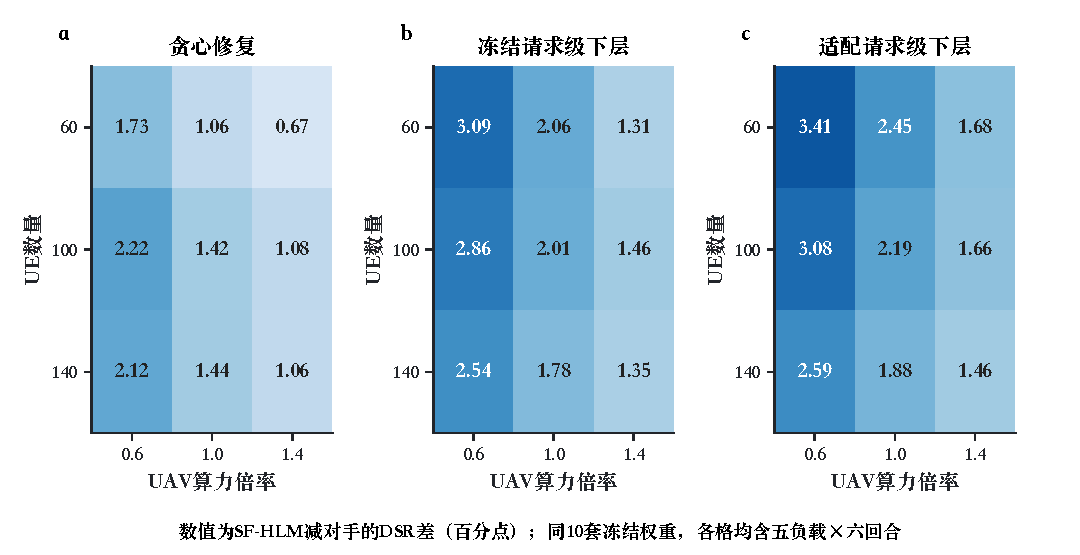
\includegraphics[width=0.98\textwidth]{../docs/figures/图5-15_九格主对手DSR差}
 \bicaption{九格学习相对三个主对手的 DSR 差。八个新格的二十四项比较统一 Holm 校正，主格保留原确认族}{DSR differences against three primary controls across nine settings, with the new 24-comparison Holm family separated from nominal confirmation}
 \label{legacy:fig:ch5-grid-differences}
\end{figure}

低算力与高负载下，贪心修复的局部选择更容易形成截止期敏感的批量，配额匹配的改善较明显。例如 $100$ UE/$0.6$ 算力下学习 DSR 为 $29.736\%$，贪心为 $27.517\%$，差 $2.219$ 个百分点，区间 $[2.051,2.387]$；$140$ UE/$0.6$ 算力差 $2.125$，区间 $[1.931,2.318]$。在 $60$ UE/$1.4$ 算力下，学习为 $50.746\%$，贪心为 $50.078\%$，差 $0.667$，区间 $[0.493,0.842]$。后者的差值区间为正，但未达到主确认事先采用的 $1$ 个百分点实用目标。

仿真环境记录的 UAV 能耗比同样随格点变化。学习相对贪心的块级比约为 $0.876$--$0.939$，各新格均低于 $1$；相对适配请求级下层在 $60$ UE/$0.6$ 算力约为 $1.0078$，没有节能但仍低于 $1.05$ 门槛。能耗还受算力平方项影响，提高计算能力可以改善时间，却可能增加实际计算能耗。因此，格点分析联合评价服务率和资源费用。

\subsection{强框架机制的场景依赖}

学习相对启发式与强随机的八格共 $16$ 项比较另组成 Holm 机制族，其中 $8$ 项通过：学习相对启发式在七个新格通过，相对强随机仅在 $140$ UE/$0.6$ 算力通过。该格学习--强随机差约 $0.355$ 个百分点，区间 $[0.150,0.560]$，Holm $p=0.0317$。其他格不能仅因未校正区间下界为正而宣称机制已稳定成立。

在 $60$ UE/$1.4$ 算力格，强随机 DSR 为 $50.772\%$，学习为 $50.746\%$，差值约 $-0.026$ 个百分点且区间跨零。结合主场景的小增量，结果表明学习额外优势依赖负载与算力，资源宽裕时强匹配框架已能取得接近学习的质量。

九格评价沿用相同观测范围和理想协调条件，刻画固定策略对规定负载与算力变化的适应程度。信息上报延迟、缺失及通信费用未随格点变化，仍是部署评价需要检验的条件。

\section{固定快照、共同 MBS 与时间预算诊断}
\label{legacy:sec:ch5-snapshot-diagnostics}

\subsection{相同状态下的真实执行复核}

为控制闭环状态差异，从 SF-HLM 的十块轨迹中，在五个负载的前两个回合分别于 $0/250/500/750$ 步采集移动前状态，共 $400$ 个快照，包含空批次。观测预测行供算法搜索，独立环境副本供最终候选分配的环境执行超时与能耗评价。两类副本保留相同几何、请求和历史状态，反事实结果不回写轨迹。

每块含 $40$ 个快照，先在块内平均，再以十个基座作配对分析。自由 MBS 的常规调用设置下，学习、启发式、强随机和贪心每快照实际超时数分别为 $10.2925$、$10.6450$、$10.3700$ 和 $10.8275$。学习--贪心差为 $-0.5350$ 个请求，区间 $[-0.6837,-0.3863]$；学习--强随机为 $-0.0775$，区间 $[-0.1989,0.0439]$。这说明共同状态下相对贪心有质量余量，相对强随机的差仍较小且不确定。

\subsection{保持共同 MBS 请求数量}

以每快照原始贪心的 MBS 请求数量为共同参照，要求初始化、修复、配额掩码、条件匹配和保底均保持这一数量，只允许改变哪些请求使用 MBS。图~\ref{legacy:fig:ch5-fixed-mbs} 对照自由和固定 MBS 结果。在固定数量下，四方法平均 MBS 请求数均为 $0.6950$，学习、强随机和贪心实际超时分别为 $10.4075$、$10.4050$ 和 $10.7875$。学习--贪心仍为 $-0.3800$，区间 $[-0.5044,-0.2556]$；学习--强随机为 $+0.0025$，区间 $[-0.0919,0.0969]$。

\begin{figure}[!htbp]
 \centering
 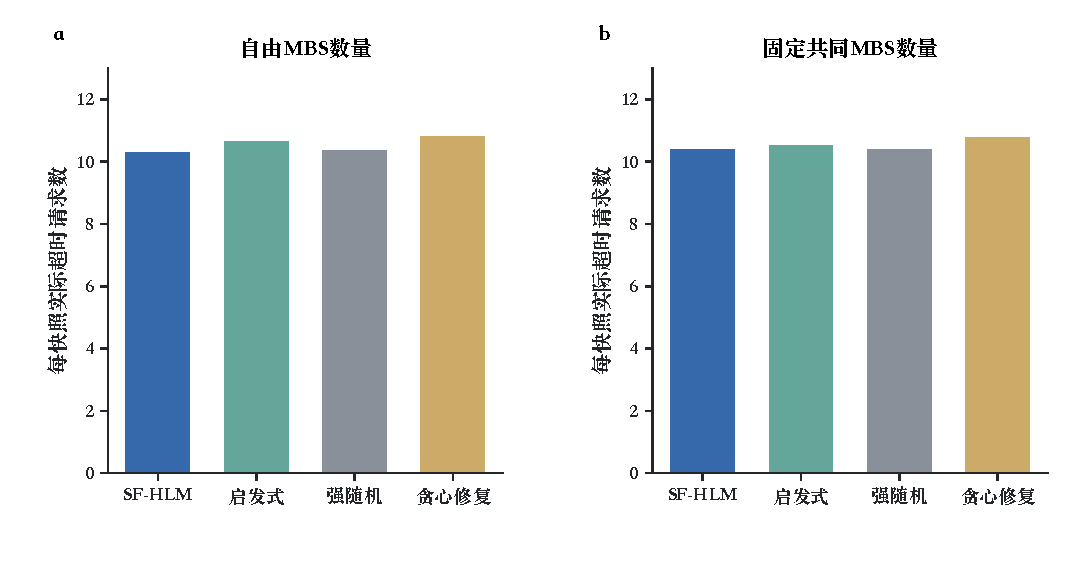
\includegraphics[width=0.98\textwidth]{../docs/figures/图5-16_自由与固定MBS快照诊断}
 \bicaption{四百固定快照的自由与共同 MBS 数量诊断。两面板分别报告自由和固定共同 MBS 数量下每快照的实际超时均值；反事实分配不回写环境，描述性均值未画误差线}{Mean actual deadline misses with free and common MBS counts on 400 snapshots; descriptive means without closed-loop write-back}
 \label{legacy:fig:ch5-fixed-mbs}
\end{figure}

固定 MBS 配额时，学习的环境分配能耗为每快照 $29619.2\,\mathrm{J}$，强随机为 $29202.0\,\mathrm{J}$，贪心为 $31637.5\,\mathrm{J}$。相对贪心，学习在相同 MBS 数量下仍减少超时和分配能耗；相对强随机，自由 MBS 时的小幅质量差在固定配额下未保留。该诊断控制单步资源使用，结果适用于相同快照，固定 MBS 约束下的长期 DSR 尚需闭环评价。

\subsection{软墙钟预算下的质量与超限}

在同一组快照施加 $20/50/100\,\mathrm{ms}$ 全路径软预算，时间从输入准备开始，包含模型推理、初始化、普通修复、搜索匹配、动作映射和消息编码。输入准备消耗先从搜索可用时间扣除；预算不足时保留合法保底。各档仍保持原在线最多 $16$ 次条件匹配与 $128$ 次普通评价，不为了时间曲线将模型的预算特征改成未经训练的无限调用值。

图~\ref{legacy:fig:ch5-wall-budget} 同时展示质量、完整时间与超限比例。三档预算下学习每快照实际超时数为 $10.6725$、$10.4250$ 和 $10.3000$，平均时间为 $22.17$、$43.65$ 和 $62.92\,\mathrm{ms}$。预算放宽时，质量接近普通调用的 $10.2925$；该实验使用同一策略在固定快照上调整执行预算。

\begin{figure}[!htbp]
 \centering
 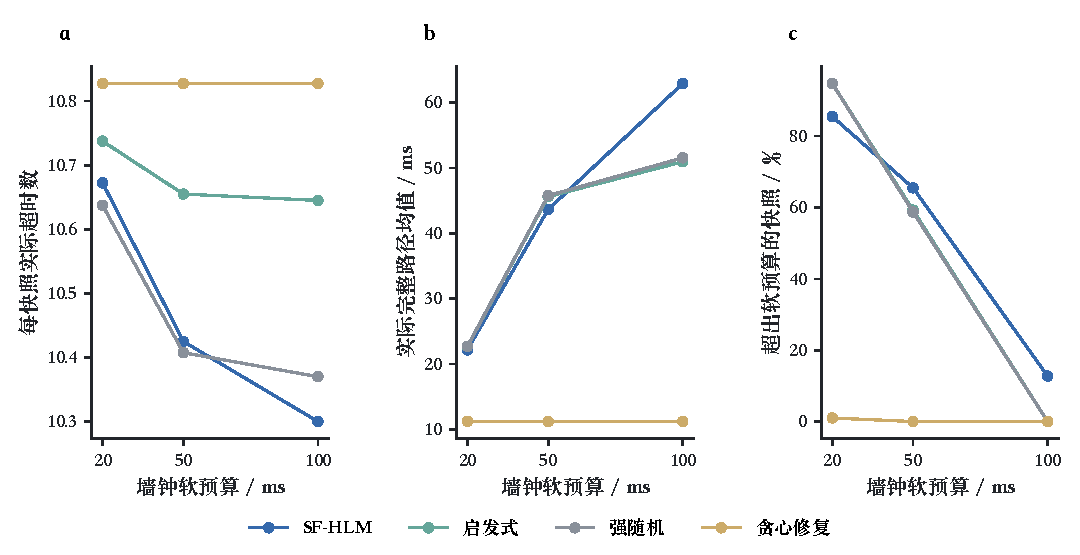
\includegraphics[width=0.98\textwidth]{../docs/figures/图5-17_墙钟预算质量时间与超限}
 \bicaption{软墙钟预算的真实质量、时间与超限率。原子匹配与完整路径开销可能越界，所有越界样本均保留}{Actual quality, time and overrun rates under soft wall-clock budgets, with all overruns retained}
 \label{legacy:fig:ch5-wall-budget}
\end{figure}

三档预算的超限快照比例为 $85.5\%$、$65.5\%$ 和 $12.75\%$，最大超限约 $7.33$、$7.06$ 和 $6.19\,\mathrm{ms}$。时间检查发生在原子匹配前，已开始的求解、动作映射与序列化仍需完成。因此预算是软截止，实际超限量与服务质量一并报告。

\subsection{匹配调用与停止行为}

图~\ref{legacy:fig:ch5-calls} 展示 SF-HLM 在十个训练块、共 $300000$ 个确认评估环境步中的调用预算使用与终止记录，包含空请求批次，平均每步使用 $11.737$ 次匹配。另在普通固定快照诊断协议下，学习平均使用 $11.255$ 次匹配，启发式 $16.000$，强随机 $15.990$；前者汇总闭环环境步，后者汇总固定快照。预算包含初始匹配，不能把调用数理解为额外迁移数。学习可在保留当前最好方案后提前 STOP，而强随机按有效非停止动作继续直到无可尝试动作或调用耗尽。停止动作与调用惩罚共同给出节约求解机会，但实际学习前向开销仍使完整软件时间高于强随机。

\begin{figure}[!htbp]
 \centering
 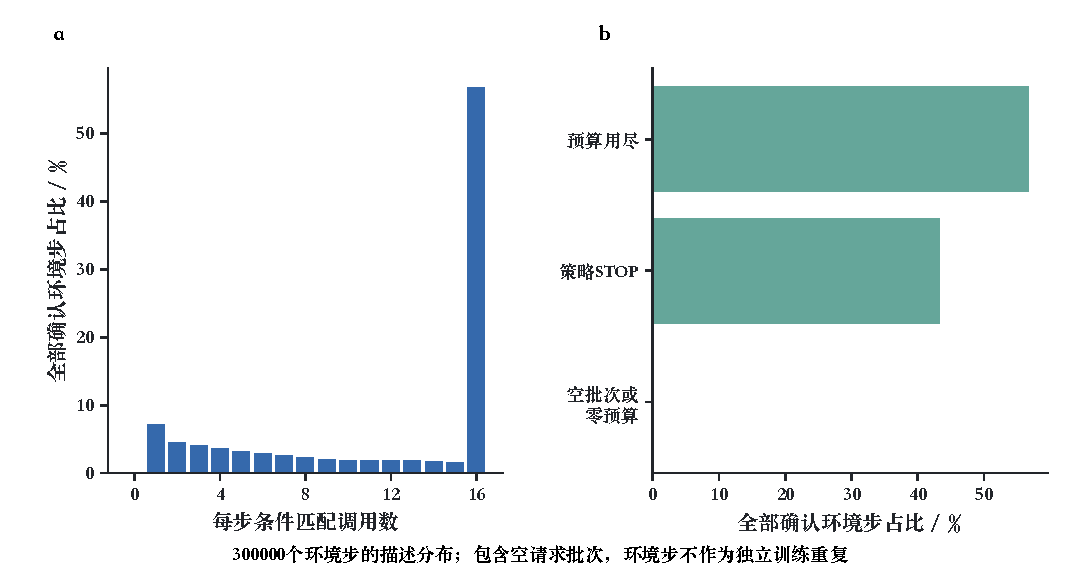
\includegraphics[width=0.98\textwidth]{../docs/figures/图5-18_匹配调用与停止行为}
 \bicaption{确认评估环境步中的匹配调用与终止行为。调用包含初始匹配及失败候选，空批次纳入统计，停止不消耗一次匹配调用}{Matching-call usage and termination behavior across confirmation evaluation steps, including initialization, failed candidates and empty batches}
 \label{legacy:fig:ch5-calls}
\end{figure}

普通快照中，学习完整平均时间约 $63.30\,\mathrm{ms}$，强随机约 $51.53\,\mathrm{ms}$；p95 分别约为 $105.24$ 和 $74.85\,\mathrm{ms}$。这一排序与确认阶段的隔离测量一致，表明搜索效率需同时考察调用数量、网络推理开销和服务质量。

\subsection{调度延迟敏感性与软件费用事后复核}
\label{legacy:sec:ch5-delay-audit}

为连接路径质量与调度费用，补充学习配额、强配额随机和贪心修复三个方法的原确认轨迹复核。每方法仍为十训练块、五工作负载、每负载六回合与每回合1000步，即每方法300回合，三方法共900回合。重放读取原卸载动作，由冻结上层重现位置决策；在请求刷新前采集实际路径时延与截止时间。逐步指标、请求计数、外生流、检查点和模型摘要均与原记录核对。该过程未训练或筛选模型，也未把新延迟回写状态。

第一类评分对所有方法施加共同附加等待 $\delta\in\{0,20,50,100,150\}\,\mathrm{ms}$，把原成功条件替换为 $T_m+\delta\leq D_m$，未接纳请求仍计入原生成分母。第二类评分按训练块、负载、回合和步号配对原隔离计时记录，使用该方法每次完整软件调用时间 $c_t$ 判断 $T_m+c_t\leq D_m$；不以平均或p95时间替代逐次费用。两类均先汇总块内成功与生成计数，再计算十块等权均值和逐项配对 $t$ 区间。它们是原轨迹上的探索性事后评分，不扩充独立训练重复数，也不改变预定主检验族。

\begin{table}[!htbp]
 \centering
 \bicaption[原轨迹的延迟及费用事后评分]{附加延迟及逐次软件费用事后评分（DSR为百分比，差值及区间为百分点）}{Post-hoc scoring with added delay and per-call software costs}
 \label{legacy:tab:ch5-delay-audit}
 \footnotesize
 \setlength{\tabcolsep}{3pt}
 \begin{tabular}{lrrrll}
  \toprule
  评分条件 & 学习 & 强随机 & 贪心 & 学习减强随机（95\%区间） & 学习减贪心（95\%区间） \\
  \midrule
  0 ms & 34.244 & 34.100 & 32.821 & $+0.143\ [0.006,0.281]$ & $+1.423\ [1.258,1.587]$ \\
  20 ms & 32.700 & 32.581 & 31.803 & $+0.119\ [-0.013,0.251]$ & $+0.897\ [0.748,1.046]$ \\
  50 ms & 30.603 & 30.506 & 30.294 & $+0.097\ [-0.029,0.223]$ & $+0.309\ [0.159,0.459]$ \\
  100 ms & 27.871 & 27.746 & 28.199 & $+0.125\ [0.017,0.232]$ & $-0.329\ [-0.498,-0.160]$ \\
  150 ms & 25.860 & 25.670 & 26.587 & $+0.190\ [0.082,0.298]$ & $-0.728\ [-0.916,-0.540]$ \\
  逐次软件费用 & 29.379 & 30.073 & 32.161 & $-0.694\ [-1.272,-0.116]$ & $-2.782\ [-3.374,-2.190]$ \\
  \bottomrule
 \end{tabular}
\end{table}

\begin{figure}[!htbp]
 \centering
 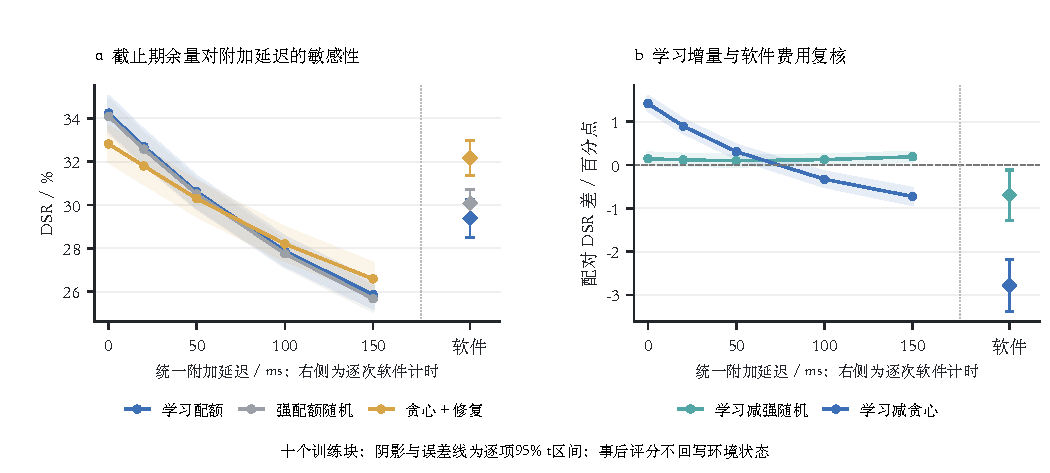
\includegraphics[width=0.98\textwidth]{../docs/figures/图5-20_调度延迟敏感性}
 \bicaption{原确认轨迹的调度延迟敏感性。左面板为DSR，右面板为学习相对强随机和贪心的配对差；菱形单独表示逐次软件费用评分，与共同延迟曲线分开。阴影与误差线为十块逐项95\% t区间，状态不回写}{Scheduling-delay sensitivity on original confirmation trajectories; diamonds denote per-call software scoring, with pointwise ten-block t intervals and no state write-back}
 \label{legacy:fig:ch5-delay-audit}
\end{figure}

零附加延迟精确复现原三方法DSR。共同等待增大后，各方法DSR下降，但差值并非固定平移：100 ms时学习减贪心为 $-0.329$ 个百分点，150 ms时为 $-0.728$，说明原学习分配的截止期余量对等待更敏感。学习对强随机的差仍较小，20和50 ms逐项区间跨零；该探索性分析不构成独立确认。

逐次软件费用评分下，学习、强随机和贪心的DSR分别为 $29.379\%$、$30.073\%$ 和 $32.161\%$。学习减强随机为 $-0.694$ 个百分点，逐项区间 $[-1.272,-0.116]$；学习减贪心为 $-2.782$，区间 $[-3.374,-2.190]$。原批次质量优势在这一费用口径下发生反转。因此，指定服务器上的软件调用门槛与计入求解等待后的服务优势须分别判断，预算受限时应把较低的软件费用纳入方法选择。

已接纳请求的路径时延超过一秒比例，学习、强随机和贪心分别约为$64.06\%$、$64.77\%$和$62.52\%$。该事后评分保留原动作与状态，不模拟等待引起的资源占用或后续反馈，不是持续队列或真实控制网络的新闭环运行。


\chapter{计费闭环确认与开发诊断的补充材料}
\label{app:cost-evidence}
\section{数据划分、参数与运行条件}
新上层种子为1520001--1520020，对应训练负载1540001--1540020；最终检查点为episode\_00199。每块在1560001--1560005五个新负载上各执行三回合，每回合1000步。原十块与开发五块均不加入本轮独立重复。固定开发HGB只有一个模型，不随新上层基座重训；本轮没有新下层PPO。

训练使用Python 3.12.11、Torch 2.6.0+cpu、NumPy 2.0.1、SciPy 1.16.0和scikit-learn 1.7.1。各新基座200回合，rollout为1000，PPO更新轮数8，batch size为256，数值线程数1。训练内部沿用purpose=pilot标签；外层独立确认由事前固定的样本隔离、方法及检验设计定义，不更改内部历史标签。

价格在原开发训练块620001--620005的400个公开状态上标定。共同能耗归一化常数为32283.910075；混合价格为0.001647731543，二值价格为0，HGB价格为0.083586671957，两个冷启动价格均为0。公开功率为回传接收0.1 W、回传发送0.5 W、UAV发送0.5 W和接收0.1 W。价格选择只比较已生成候选，不重求带价格边成本的匹配。

\section{全部参照与固定潜在分母}
\begin{table}[!htbp]
\centering
\bicaption{新确认全部参照的配对差与能耗比}{All paired contrasts and energy ratios in the new confirmation}
\label{tab:cost-all-contrasts}
\small
\begin{tabular}{lrrr}
\toprule
参照 & 计费DSR差/百分点及95\%区间 & 正向块 & 平均块能耗比\\
\midrule
G & $1.02828\ [0.93660,1.11997]$ & 20/20 & 1.01866\\
R10 & $0.66280\ [0.56046,0.76513]$ & 20/20 & 1.11228\\
R16 & $0.69841\ [0.63499,0.76183]$ & 20/20 & 1.13630\\
二值价格 & $0.26243\ [0.16518,0.35968]$ & 18/20 & 1.08299\\
未加价混合 & $0.00243\ [-0.05916,0.06402]$ & 9/20 & 0.91278\\
冷启动先验 & $0.04960\ [-0.03930,0.13850]$ & 10/20 & 0.91296\\
冷启动半概率 & $-0.02341\ [-0.10614,0.05932]$ & 9/20 & 0.91537\\
固定HGB & $0.69612\ [0.60433,0.78790]$ & 20/20 & 0.92201\\
\bottomrule
\end{tabular}
\end{table}
表~\ref{tab:cost-all-contrasts}中差值为主候选减参照，能耗比为候选除以参照；区间为逐项配对$t$区间，并非同时置信区间。只有G和二值价格属于预定两项主比较，其余六项为描述性分析。主比较精确符号翻转双侧$p$分别为$1.90735\times10^{-6}$与$1.52588\times10^{-5}$，依赖独立块配对效应的对称性，不能解释为无假设的因果随机化检验。

各方法共同潜在服务请求总数为9,215,840。保留原成功数、替换分母后，候选减G为$1.02892$个百分点，95\%配对$t$区间$[0.93627,1.12158]$；候选减二值价格为$0.26295$个百分点，区间$[0.16552,0.36038]$。这只检验轻微实际服务分母变化，既不改变原主指标，也不模拟低电量UE继续生成服务请求的反事实运行。

\section{复现入口与核验覆盖}
本轮冻结统计位于仓库\path{results/sf_hlm_learning_feasibility_20261016/}\allowbreak\path{framework_confirmation_20261018/confirmation_saturated120_v1/analysis/summary.json}；同目录的\path{protocol.json}、\path{raw_audit.json}分别给出冻结协议和原始核验。程序报告与180条块乘方法计数表位于原任务\path{validation/framework_confirmation_20261018/evidence_saturated_v1/formal/}下的\path{report.md}与\path{block_metrics.csv}。源码精确执行副本为原任务\path{assets/releases/framework_saturated_425716b43b76/}。历史服务器绝对路径作为溯源保留，本机相应资料按仓库相对路径同步。

全部2,700,000步完成请求阈值、计数、时间窗口、配额预算、预测能耗筛选及配对外生流核验；预先选定的180回合、180,000步及1,984,786个请求另做原Env物理重放。后者使用原动作和原实测时钟，不重新计费。二者覆盖不同，不能称2700回合全部物理复现。训练直接审计检查20个不同上层权重指纹、全部4000训练回合及最终检查点。上述工作属于主代理自审，不是独立同行评审。

\section{历史缓存学习开发诊断与停止依据}
\label{sec:cost-development-diagnostics}
本节复述已封存的开发报告，不新增拟合或统计检验。样本来自五个历史上层训练块的400个固定状态，共13,459条协作边；私有邻机缓存仅用于离线标签和物理评分，不进入在线选择器。该条件缓存学习模型与本章正式确认中的固定HGB参照不是同一方法。状态、边、交叉验证折及延迟分支均不增加独立训练块数，以下只作开发描述。

在既有学习模型、冷启动半概率及冷启动先验三种方法所选配额定义的共同10 ms敏感边并集中，8,071条边的学习Brier为0.043477，冷启动先验和冷启动半概率分别为0.051185、0.062105；学习已选的1,671条敏感边上，三者分别为0.037617、0.046621和0.067472。子集沿用原状态权重，未重新归一为子集状态等权。尽管这些预测误差较低，学习模型相对冷启动半概率的任务DSR仍低约0.09992个百分点。

\begin{table}[!htbp]
\centering
\bicaption{历史开发快照中的分配关系与服务差贡献}{Assignment relationships and service-difference contributions in historical development snapshots}
\label{tab:cost-development-decomposition}
\small
\begin{tabular}{lrr}
\toprule
学习与冷启动半概率的分配关系 & 状态数 & 共同10 ms贡献/百分点\\
\midrule
完全相同分配 & 171 & 0.000000\\
同配额、不同请求身份 & 125 & 0.007686\\
不同配额 & 104 & $-0.107610$\\
\bottomrule
\end{tabular}
\end{table}

表~\ref{tab:cost-development-decomposition}按原报告将服务差分为互斥三类，未舍入贡献可加回原比较，不是各类自身成功率之和。负贡献主要来自不同配额状态，但没有随机化候选生成或能耗筛选，不能识别唯一失败原因。

\begin{table}[!htbp]
\centering
\bicaption{已完成的缓存学习开发支线及停止依据}{Completed cache-learning development branches and their stopping criteria}
\label{tab:cost-development-stops}
\small
\begin{tabularx}{\textwidth}{p{0.16\textwidth}YY}
\toprule
开发支线 & 封存观察 & 预定判定及证据范围\\
\midrule
条件缓存匹配 & 共同10/20 ms下相对最好无标签参照分别为$-0.09992$/$-0.04612$个百分点 & 未过质量、方向及能耗联合门槛；不进入原生计时与闭环\\
同池学习重排 & 共同10 ms增益0.03843个百分点，逐项95\% $t$区间$[-0.02001,0.09688]$；20 ms区间也跨零 & 未达到10/20 ms均至少0.1个百分点等联合要求；未作独立确认\\
增加公开时延差特征 & 留出Brier改善0.00013144，五块均正 & 小于预定0.001门槛；在预测阶段停止，未进行任务匹配或计时\\
\bottomrule
\end{tabularx}
\end{table}

同池重排只改变共同公开候选池中的选择；额外特征仅为公开命中与未命中基时延差的对数变换。表~\ref{tab:cost-development-stops}的共同延迟不是各方法实测费用，五块区间为开发描述，不并入新确认主检验族。停止结论只针对相应冻结方案，不推出其他学习方法均无效。

400状态中100个来自step0，其1,980条协作边命中率为0；其余11,479条边按原状态权重的命中率为93.6962\%。原状态等权使step0占预测指标的25\%，不能代表完整1000步回合的时间分布，也未确认当前解析方法的长回合信息价值。

复现来源为仓库\path{output/sf_hlm_learning_feasibility_20261016/}\allowbreak\path{deliverables/}中的\path{cache_decision.md}、\path{cache_context.md}、\path{cache_regime_matching.md}、\path{cache_guarded_rerank.md}及\path{cache_gap.md}；各报告链接相应冻结协议、JSON和自审记录。

\section{当前解析方法的长回合与迁移开发补证}
\label{sec:cost-stage-b-development}

本节采用五个历史上层开发基座620001--620005，以及经历史登记清单核验的新开发负载19271001--19271003。价格和能耗归一化常数沿用原解析方法，在效果揭示前冻结。五场景四方法共300回合；中心场景另补二值零价、解析零价及共同价格二值各15回合，复用原解析方法作为共同价格解析组，实际共345个不同回合、345000步。独立描述单位仍为五个上层块，各块先合并计数求率；本节所有区间均为逐项95\%配对$t$描述区间，不加入原二十块确认的主检验族。

本轮使用最多32个单线程工作进程，分配至不同物理核；共享服务器另有背景负载，不是系统级独占。每步按原完整软件调用时间注入请求时延，随后形成奖励与下一观测；磁盘日志在计时外。新费用条件与原120核确认分开，不能拼接计算加速比。全量逐步计费、请求计数、预算、摘要和配对流核验通过；另在1228个抽样源状态复现原物理时延，并按原逐次费用复核成功数。

\subsection{代表性抽样与评分--价格模块干预}

G和解析方法各15个1000步源回合，每回合分40个等长区间，各区间在效果前随机抽一步，共1200个主状态；另外28个step0只作附加冷启动，不重复计权。全部合法协作边的私有缓存标签由独立离线过程读取，候选生成与选择只接收原公开rows。解析所选配额下五块关键边比例为$63.231\%$、$66.306\%$、$60.974\%$、$57.787\%$、$59.473\%$，分母为目标配额大于零的合法协作边，不能解释为关键边稀少。暖态的原先验Brier为0.053057，冷启动半概率为0.065153；全边log loss分别为0.571406与0.510248，两类预测误差的排序并不一致，也未比较新学习模型。

四组以二值模块或解析模块执行配额内指派，再以零价或共同冻结价格选择候选。共同$\lambda=0.0016477315429376078$，归一化常数为32283.91007507；各组共享初值、普通修复、提议顺序、十次总匹配预算、预测筛选与反馈。二值和混合的配额内能耗项尺度也不同，故这是评分--指派模块干预，而非仅替换概率公式。表~\ref{tab:cost-stage-b-components}同时保留固定快照与闭环比较。

\begin{table}[!htbp]
\centering
\bicaption{共同价格下的开发组件比较；差值单位为百分点}{Development module comparisons under a common price; differences in percentage points}
\label{tab:cost-stage-b-components}
\small
\begin{tabular}{lrrr}
\toprule
比较 & 固定状态共同10 ms & 计费闭环 & 闭环能耗比\\
\midrule
$M_0-B_0$ & $0.196\ [0.108,0.283]$ & $0.262\ [0.028,0.496]$ & 1.1250\\
$M_\lambda-B_\lambda$ & $0.111\ [0.026,0.195]$ & $0.251\ [-0.498,0.999]$ & 1.0523\\
$B_\lambda-B_0$ & $0.000\ [0.000,0.000]$ & $0.002\ [-0.005,0.009]$ & 1.0000\\
$M_\lambda-M_0$ & $-0.085\ [-0.125,-0.045]$ & $-0.009\ [-0.721,0.703]$ & 0.9356\\
\bottomrule
\end{tabular}
\end{table}

表中$B$、$M$分别指二值、解析模块；固定状态列等权合并G与解析源轨迹，各状态锁定同一上层motion并用原物理环境评价分配，不能当作原生闭环增益。共同带价模块差在G源状态为$-0.028\ [-0.090,0.035]$，在解析源状态为$0.247\ [0.059,0.435]$，显示状态来源依赖。共同价格没有改变本批固定状态的二值最终分配，闭环极小DSR差伴随相同接纳与能耗；不把它归为价格的任务增益。解析加价的闭环DSR区间跨零，能耗比仅作描述，不能据此宣称无损节能。

原公开分解未由私有时延校正。主样本源策略所选协作边中，11898条完成公开反演残差核对，9条绝对残差大于$10^{-6}$秒，均在$p\ge1-10^{-10}$组；最大残差约$2.76\times10^{-4}$秒。此处保留数值近似，不把未回退等同于物理精确。候选并集、失败筛选原因、三类分配贡献和完整概率误差另存原始结果。

\subsection{五场景零调参迁移及边界}

图~\ref{fig:cost-stage-b-transfer}分别改变UE数或UAV算力，其余物理参数、原上层权重、价格和归一化常数不变。上层仍保留每机30个UE槽及原排序，$140$ UE可能被观测截断；下层请求槽未触发容量错误。解析相对G的均差在五场景均为正，但高负载和高算力各有负向块；解析相对二值的五个区间均跨零。只覆盖十字而非完整交互网格，也没有新增上层训练块。

本轮在开发补证后停止，独立新基座与跨因素交互仍需新设计。协议、种子、原始记录及统计见\path{results/chapter5_followup_20261027/}\allowbreak\path{development_v2/}；本节不与旧400状态或二十块主确认合并。

\begin{figure}[!htbp]
\centering
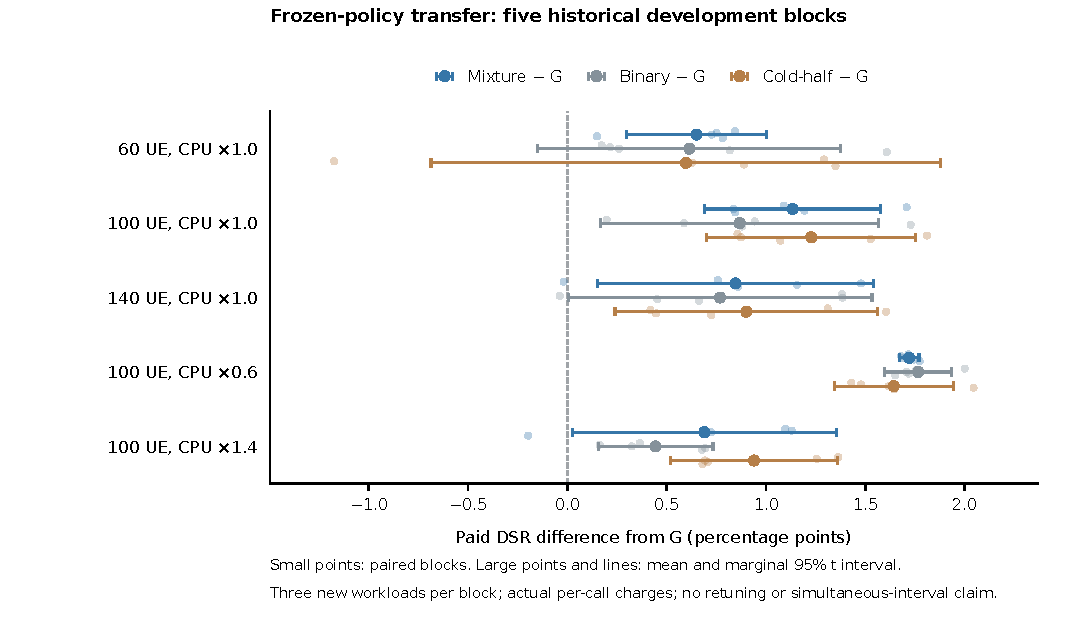
\includegraphics[width=0.98\textwidth]{../docs/figures/chapter5_stage_b_20261027/stage_b_transfer.pdf}
\bicaption{冻结策略的五场景开发迁移。小点为五个历史块配对差，大点及线为均差与逐项95\%配对$t$区间；各块合并三个新负载回合}{Five-setting development transfer of frozen policies; paired historical blocks, means and marginal 95\% paired t intervals}
\label{fig:cost-stage-b-transfer}
\end{figure}
